% CVPR 2027 submission -- AlignFormer as a plug-in. Template: https://github.com/cvpr-org/author-kit
%
% Top of this file: the NEW paper, currently an outline (highlights per paragraph, empty table shells).
% Bottom of this file: the OLD draft of Oct 22, kept for reference only. Delete that block before submitting.

\documentclass[10pt,twocolumn,letterpaper]{article}

%%%%%%%%% PAPER TYPE  - PLEASE UPDATE FOR FINAL VERSION
% \usepackage{cvpr}              % To produce the CAMERA-READY version
\usepackage[review]{cvpr}      % To produce the REVIEW version
% \usepackage[pagenumbers]{cvpr} % To force page numbers, e.g. for an arXiv version

% Import additional packages in the preamble file, before hyperref
%% Packages and macros for the AlignFormer draft. Loaded before hyperref.

\usepackage{graphicx}
\usepackage{amsmath,amssymb}
\usepackage{booktabs}
\usepackage{multirow}
\usepackage{xspace}
\usepackage{xcolor}
\usepackage{siunitx}
\usepackage{tikz}
\usetikzlibrary{fit,positioning,arrows.meta,backgrounds,calc}
\sisetup{detect-all}

%% Inline annotations. Disable for submission by uncommenting the two lines below the definitions.
\newcommand{\red}[1]{{\color{red}#1}}
\newcommand{\todo}[1]{{\color{red}#1}}
\newcommand{\TODO}[1]{\textbf{\color{red}[TODO: #1]}}
% \renewcommand{\TODO}[1]{}
% \renewcommand{\todo}[1]{#1}

%% Placeholder for a figure that is not drawn yet: \placeholderfig{<width>}{<height>}{<what will go here>}
\newcommand{\placeholderfig}[3]{%
  \fbox{\begin{minipage}[c][#2][c]{\dimexpr#1-2\fboxsep-2\fboxrule\relax}\centering\small\color{red}#3\end{minipage}}}

%% Names
\newcommand{\paper}{AlignFormer\xspace}
\newcommand{\freealign}{FreeAlign\xspace}
\newcommand{\vxreal}{V2X-Real\xspace}
\newcommand{\opvv}{OPV2V\xspace}

%% Math
\DeclareMathOperator*{\argmin}{arg\,min}
\DeclareMathOperator*{\argmax}{arg\,max}
\newcommand{\R}{\mathbb{R}}
\newcommand{\SE}{\mathrm{SE}(2)}
\newcommand{\ap}[1]{AP$_{#1}$}

%% Tables: a pending number
\newcommand{\pending}{{\color{red}--}}
\newcommand{\best}[1]{\textbf{#1}}

%% work harder in optimizing text layout; enable at the very end
% \usepackage{microtype}

%% ---- Outline macros (scribble stage). Remove with the outline. ----
\definecolor{outlineblue}{rgb}{0.05,0.25,0.55}
\definecolor{outlinegreen}{rgb}{0.0,0.42,0.2}
\definecolor{outlineorange}{rgb}{0.72,0.33,0.0}
\newcounter{parano}[section]
%% \para{what this paragraph is}{its highlights}: one call = one paragraph of the final paper
\newcommand{\para}[2]{\par\smallskip\noindent\stepcounter{parano}{\color{outlineblue}\textbf{\P\arabic{parano}\ #1.}} #2\par}
%% \budget{...}: length this section may take
\newcommand{\budget}[1]{\par\noindent{\small\itshape\color{gray!60!black}Budget: #1}\par}
%% \code{...}: the code this paragraph describes. \exists = it exists today; \tobuild = it must be written first
\newcommand{\code}[1]{{\footnotesize\color{outlinegreen}\ [code: \texttt{\detokenize{#1}}]}}
\newcommand{\tobuild}[1]{{\footnotesize\color{outlineorange}\ [to build: \texttt{\detokenize{#1}}]}}
%% \claimref{C1}: the claim from the glance table this paragraph carries
\newcommand{\claimref}[1]{{\footnotesize\bfseries\color{red!70!black}\ [#1]}}
\newcommand{\oldbanner}{{\centering\LARGE\bfseries\color{red}OLD DRAFT (Oct 22)\\\large reference only, not part of the new paper\par}\bigskip}
\definecolor{outlineteal}{rgb}{0.0,0.5,0.5}
%% \why{...}: why this table or figure exists and what we conclude from it. Remove with the outline.
\newcommand{\why}[1]{\par\smallskip{\footnotesize\raggedright\color{outlineteal}#1\par}}


\definecolor{cvprblue}{rgb}{0.21,0.49,0.74}
\usepackage[pagebackref,breaklinks,colorlinks,allcolors=cvprblue]{hyperref}

%%%%%%%%% PAPER ID  - PLEASE UPDATE
\def\paperID{*****} % *** Enter the Paper ID here
\def\confName{CVPR}
\def\confYear{2027}

%%%%%%%%% TITLE (working title)
\title{AlignFormer: A Plug-in Pose Corrector for\\Late and Intermediate Cooperative Perception}

%%%%%%%%% AUTHORS (anonymised for review; the review option hides this block)
\author{Anonymous CVPR submission\\
Paper ID \paperID
}

\begin{document}
\maketitle
\sloppy

%%%%%%%%% THE NEW PAPER (outline)
%% The one-page contract of the paper. Not part of the final paper.
\section*{Read first: the paper at a glance}

\noindent\textbf{Thesis.} Every cooperative pipeline, late or intermediate, places a CAV's data through one CAV-to-ego transform. AlignFormer corrects that transform from detected boxes and each vehicle's own odometry, then hands it to the unchanged host. No host retraining, and no knowledge of the noise. The method is Propose, Verify, Abstain: a transformer over box tokens with Sinkhorn assignment and a closed-form pose proposes, an exact RANSAC fit verifies, and a Wald test on the estimator's own covariance decides whether to correct at all. It then follows each CAV over time and, in late fusion, estimates delay.

\medskip\noindent\textbf{Rules of this paper.}
\begin{itemize}\setlength\itemsep{1pt}
  \item[\textbf{R1}] \textbf{No noise knowledge.} The plug-in never receives the noise level, its distribution, the delay, or any ground truth. Only the simulator that corrupts the poses knows them. A result obtained any other way is not reported.
  \item[\textbf{R2}] \textbf{Paper equals code.} Every method paragraph names the code that does it. Every number names its run. A claim without a run is not written.
  \item[\textbf{R3}] \textbf{One configuration.} Hyper-parameters are chosen once on V2X-Real validation, then frozen for all datasets, hosts and conditions.
  \item[\textbf{R4}] \textbf{One protocol.} Same frames, ego, ground-truth window, noise draws and evaluator for every method on a dataset.
  \item[\textbf{R5}] \textbf{Only necessary runs.} Every run feeds one exhibit below. No exhibit, no run.
  \item[\textbf{R6}] \textbf{Stages must earn their place.} A stage that does not help in the ablation is removed from the method and the code.
\end{itemize}

\medskip\noindent\textbf{How to read the outline.} Each \textcolor{outlineblue}{\textbf{\P n}} is one paragraph of the final paper, with its highlights. \textcolor{outlinegreen}{\footnotesize[code]} is code that exists today, \textcolor{outlineorange}{\footnotesize[to build]} is code to write first, and \textcolor{red!70!black}{\footnotesize\textbf{[C$n$]}} is the claim it carries. \textcolor{outlineteal}{Teal text} under an exhibit says why it exists and what we conclude from it. Tables are empty shells: their rows and columns are what the experiments must produce. The ledger at the end maps each exhibit to its run.

\begin{table*}[t]
  \centering\small
  \raggedright\textbf{The six claims.} The experiments exist only to test these. ``Publishable if'' is fixed now, before any number is seen; ``if not'' says what the paper then says instead.\par\medskip\centering
  \begin{tabular}{@{}l p{5.6cm} l p{4.6cm} p{4.0cm}@{}}
    \toprule
    & Claim & Exhibits & Publishable if & If not \\
    \midrule
    \textbf{C1} & \textbf{It is the better plug-in for intermediate fusion.} On the same unchanged hosts and noise draws, it recovers more AP than FreeAlign and does not damage the clean case. \emph{Headline, and the go/no-go.} & T1, F3, F4 & At $\sigma\geq 0.4$: above FreeAlign on most hosts with paired significance, and at least 90\% of perfect-pose AP on OPV2V and V2X-Real at $\sigma=1$. At $\sigma=0$: within 0.02 of perfect pose. & If level with FreeAlign, the headline moves to late fusion and the clean case (C3), and T1 is reported as parity. \\
    \textbf{C2} & \textbf{It can replace a network's built-in correction.} Same weights, only the corrector changes: CoAlign's pose graph, RoCo's matching. & T2 & At or above the built-in correction at $\sigma\geq 0.4$. & Claim ``competitive, and no network-specific stage''. \\
    \textbf{C3} & \textbf{It beats FreeAlign in late fusion} at every $\sigma$ on OPV2V and V2X-Real, with Propose, Verify, Abstain alone (one frame) and over time. & T3, T4 & Paired difference positive in every cell over 20 seeds, at AP$_{0.7}$ and AP$_{0.5}$. & Name the cells where it does not. \\
    \textbf{C4} & \textbf{It uses the reported pose safely, with no noise knowledge.} FreeAlign needs none either, because it does not use that pose. Ours does, so a bad report must not hurt it. The frozen configuration holds under noise it never saw. & T5 & Above FreeAlign in every row. The out-of-training-range row may fail if Abstain contains the damage. & State the limit as a limitation. \\
    \textbf{C5} & \textbf{It handles unknown delay in late fusion.} Pose and latency are recovered from boxes, and zero delay is unharmed. & T6, F5 & Above both FreeAlign rows at 100--400\,ms, and at most 0.005 below the no-delay-stage result at 0\,ms. & Drop the stage (R6) or restrict the claim to where it holds. \\
    \textbf{C6} & \textbf{Each stage earns its place, and the cost is negligible.} & T7 & Each stage helps on at least one dataset and hurts on neither. Message below 0.01\% of a host's. & Remove the stage (R6). \\
    \bottomrule
  \end{tabular}
\end{table*}

\clearpage

\section*{Abstract}
\budget{1 paragraph, about 200 words. Written last, from final numbers.}

\para{The one abstract paragraph}{Six moves, in this order:
\begin{enumerate}\setlength\itemsep{0pt}
  \item \textbf{Problem.} Cooperative perception trusts each CAV's reported pose. When that pose is wrong, late and intermediate fusion both collapse, sometimes below the ego alone.
  \item \textbf{Gap.} Remedies built into one network need its training. Plug-ins exist (FreeAlign), but they treat each frame alone, do not use the reported pose when it is right, and leave motion under delay to a separate network.
  \item \textbf{Ours, stated first as a plug-in.} AlignFormer is a plug-in. It sits in front of fusion and outputs one corrected transform per CAV. Hosts are unchanged and not retrained. It is told nothing about the noise or the delay.
  \item \textbf{How, one or two sentences.} Propose, Verify, Abstain: a transformer with Sinkhorn assignment and a closed-form pose, an exact RANSAC fit, and a Wald test that decides whether to correct at all. Pooled over time through each vehicle's odometry.
  \item \textbf{Results.} Intermediate hosts keep $N$\% of their clean AP, against $M$\% uncorrected and $K$\% with FreeAlign \claimref{C1}. It beats FreeAlign in late fusion on simulated and real-world data \claimref{C3}, and under unknown delay \claimref{C5}.
  \item \textbf{Cost.} $B$ bytes per frame and $T$\,ms \claimref{C6}.
\end{enumerate}}

\section{Introduction}
\budget{1 page, 5 paragraphs.}

\para{The problem}{Sharing data across vehicles extends perception beyond line of sight, but only if the sender's pose is right. Open with one measured collapse from each fusion family, both at the same noise level (Table~T1 uncorrected, Table~T3 uncorrected), and the fact that uncorrected fusion can fall below the ego alone.}

\para{What exists, with credit}{Plug-in correction already exists, and we say so. FreeAlign (box graph matching) and RoCo (object matching and pose graph) both claim to work with existing hosts without retraining. NEAT is a plug-in that aligns features but trains with the host. CoAnchor uses object anchors and short box histories under spatio-temporal misalignment, as its own framework, with the delay given. Credit them plainly.}

\para{The question this paper asks}{Whatever the fusion family, the pose acts through one CAV-to-ego transform, which is why a plug-in can work at all. So the question is not whether to build a plug-in, but what a good one must do. What existing plug-ins leave on the table: hand-built matching declines pairs with few shared objects, and an exact fit is only as good as its hard matches; nothing tests whether a correction should be applied, so the clean case is damaged; each frame is solved alone; and in late fusion nothing compensates object motion under delay (FreeAlign leaves that to a trained network on feature maps, SyncNet). This is the paper's central paragraph.}

\para{Our solution}{AlignFormer as a plug-in (Fig.~F1). What goes in: boxes, reported pose, own odometry. What comes out: one corrected transform per CAV. What it is never told: noise level, distribution, delay. One sentence on each stage, each answering one of the three gaps above. Same module, same weights, no host retraining.}

\para{Contributions}{A short list, each bullet tied to a claim and an exhibit:
\begin{itemize}\setlength\itemsep{0pt}
  \item Propose, Verify, Abstain from boxes alone: a transformer with Sinkhorn assignment and a closed-form pose proposes, an exact fit verifies, and a Wald test on the estimator's own covariance decides whether to correct at all \claimref{C3, C6}.
  \item The same pipeline over time, with no knowledge of the noise: measurements carried by each vehicle's odometry, robust pooling, and an online decision to keep or override the reported pose \claimref{C3, C4}.
  \item A plug-in for unchanged hosts: above FreeAlign on the same $N$ intermediate hosts on OPV2V and V2X-Real, and able to replace built-in correction \claimref{C1, C2}.
  \item Joint pose and latency estimation from boxes, with an observability test, for late fusion under unknown delay \claimref{C5}.
  \item One protocol: same frames, noise draws and evaluator across all methods, reported with paired statistics.
\end{itemize}}

\section{Related Work}
\budget{0.5 page, 4 paragraphs. Each ends by saying what is different here. References checked before writing.}

\para{Intermediate fusion under pose error}{Attention and transformer hosts (AttFuse, V2X-ViT, CoBEVT, Where2comm, CoST) gain robustness, if at all, through training with noise. They remain our hosts. \emph{Difference:} we do not compete with them, we repair them.}

\para{Pose correction built into a network}{Vadivelu et al., CoAlign's pose graph, MRCNet, SparseAlign's PoseAlign (learned pose-agnostic box features, then a pose graph), CoRA, FeaKM, V2VLoc. RoCo's matching and pose graph, which claims integration without retraining, single frame, with a distance gate. \emph{Difference:} tested on many unchanged hosts, and compared with CoAlign and RoCo directly in Table~T2 on the same weights.}

\para{Alignment from boxes, and plug-ins}{FreeAlign: graph matching, plugs into hosts without retraining, works without GNSS (its paper mentions checking GNSS reliability in passing). Its limits: degenerate below three shared objects, exact fit only as good as its hard matches. OptiMatch's optimal-transport matching for object-level correction. \emph{Difference:} learned association plus exact verification, pooled over time, using the reported pose when the evidence supports it.}

\para{Delay and time}{Latency compensation with known or separately estimated delay (SyncNet, CoBEVFlow). FreeAlign's clock search, which leaves motion to SyncNet on feature maps, so late fusion gets none. NEAT absorbs delay implicitly in features. CoAnchor and SparseAlign use short histories, CoAnchor with the delay given. \emph{Difference:} the delay is estimated jointly with the pose, from boxes and sender velocities, and tested for observability.}

\section{System Model}
\label{new:sec:system}
\budget{0.5 page, 5 paragraphs, Fig.~F1. This section defines the solution's contract, so it must match the code exactly.}

\begin{figure}[t]
  \centering
  \placeholderfig{\linewidth}{3.2cm}{\textbf{F1: the plug-in.} One box in front of fusion. Top path: late fusion (CAV boxes $\to$ transform $\to$ NMS). Bottom path: intermediate fusion (CAV points or features $\to$ transform $\to$ host). The same corrected transform feeds both. Marked ``unchanged'': the hosts. Drawn in TikZ, no run needed.}
  \caption{\textbf{F1.} AlignFormer sits in front of any fusion family and changes only the CAV-to-ego transform.}
\end{figure}

\para{Setting}{One ego and $N$ cooperating agents, each detecting in its own frame and sending a message with its reported pose. One ego-CAV pair at a time; several CAVs repeat it. Notation for the reported transform $N_t$ and the true transform.}

\para{The one transform}{Where the transform acts in each family: late fusion places boxes with it; intermediate with \texttt{proj\_first} projects points before voxelization; intermediate without it warps features. Three code paths, one matrix. This is what makes a plug-in possible, and the section's key point. \code{OpenCOOD transformation_matrix, pairwise_t_matrix} \tobuild{plugin hook}}

\para{What can go wrong}{The reported pose has an error of unknown form. The message may be old by an unknown delay. Only a planar rigid error is modelled (translation and yaw); height, roll and pitch are left to the detector. The ego's own pose is the reference frame.}

\para{What the plug-in may see (R1)}{Stated plainly as a list. \emph{Allowed:} both agents' boxes and scores; the reported pose; each vehicle's own LiDAR odometry; sender velocities from its own tracker. \emph{Never:} noise level or distribution, the delay, ground truth, correspondences, host internals, or any retraining. This paragraph is the paper's promise, and every experiment obeys it.}

\para{Problem statement}{For each CAV and frame, causally (past and present only), output a corrected transform and hand it to the unchanged host. Success is measured by the host's AP, with pose error reported as the explanation, not the goal.}

\section{AlignFormer}
\label{new:sec:method}
\budget{2 pages, 13 paragraphs, Fig.~F2. Each paragraph describes code that runs in the final experiments, nothing else (R2).}

\begin{figure}[t]
  \centering
  \placeholderfig{\linewidth}{2.8cm}{\textbf{F2: the pipeline.} Per frame: Propose $\to$ Verify. Over time: carry by odometry $\to$ robust pooling $\to$ online Abstain $\to$ corrected transform. Late fusion only: latency fit and staleness score. Drawn in TikZ, no run needed.}
  \caption{\textbf{F2.} The stages. Nothing in the pipeline reads a noise level.}
\end{figure}

\subsection{Overview}
\para{The whole pipeline in one paragraph}{Input, stages, output, each in a sentence, following Fig.~F2. Repeat that no stage reads a noise level.}

\subsection{One frame: Propose, Verify, Abstain}
\para{Propose}{A small transformer over box tokens, Sinkhorn soft assignment with dustbins for unshared objects, and a closed-form, heading-augmented, inverse-variance-weighted Kabsch pose, with two robust reweighting steps. Differentiable end to end, so the matcher is trained on the pose it produces. Trained once per dataset, separately from any host; the host's training is untouched. Declare the training noise range ($\leq 2$\,m) here; T5 tests beyond it. \code{alignformer_pva}}

\para{Verify}{An exact re-solve: mutual nearest neighbours under the proposed pose, shrinking gates, RANSAC. Heading plays no part in the fit, a choice confirmed on validation. \code{verify_core, variants.alignformer_c}}

\para{Abstain}{Should this pair be corrected at all? A Wald test of the proposed correction against no correction, using the covariance the weighted solve implies and a fitted noise model for the detections, so it needs no noise level. An agreement rule between the proposal and the exact fit, with a consensus floor, decides which fit to keep. \code{abstain.py, verify_core}}

\para{Why all three}{The soft fit is never catastrophically wrong, the hard fit is sharp when its matches are right, and the test protects the case where no correction is needed. Short, with the evidence in T4 and T7.}

\subsection{Over time}
\para{Carrying measurements}{Each frame gives a measurement of the CAV's pose. Both vehicles' odometry carries it to the current frame, with its covariance propagated through exact Jacobians. Odometry is real LiDAR odometry from each vehicle's own scans, with a fixed published accuracy, never the simulator's. \code{temporal._carry} \code{odometry.py, build_odometry_table.py}}

\para{Robust pooling}{Generalised least squares over a 30-frame window. Carried measurements share odometry, so they are correlated, and the estimator models that. Outliers are down-weighted by a Cauchy kernel. Measurement noise is estimated online from consecutive differences, so nothing is assumed about it. \code{temporal._robust_gls_agreement, temporal._NoiseScale}}

\subsection{Abstain over time}
\para{When to keep the reported pose}{The per-frame test sees one frame; this one sees the window. It is a choice between two estimates: the reported pose and the window's. The window is applied if most of its measurements agree with it, or if its spread is below the reported pose's error level, which is itself estimated online from past gaps. No threshold depends on the noise level. \code{temporal.temporal_decisions, consistency="adaptive"}}

\subsection{Delay (late fusion)}
\para{Why delay is a different problem}{A delay moves objects by their own velocity, so the error is no longer rigid and no single transform can fix it. Without a motion model, alignment fits the moving objects' displacement and misplaces the rest.}

\para{Joint pose and latency}{Fit pose and latency together from matched boxes and the sender's velocities. An F-test decides whether a delay exists, and velocity diversity measures whether it is observable at all; identical motion is indistinguishable from a translation. Estimates are pooled per CAV before testing. \code{latency.joint_fit, latency.refine_latency}}

\para{Staleness-aware scores}{Scale each delayed box's score by the probability its predicted position stays within the IoU tolerance, using the sender's own tracking errors. Tracker and table use the same real odometry, and the table is fitted on validation frames. \code{fusion.staleness_confidence} \tobuild{tracker on real odometry, validation table}}

\subsection{Plugging in}
\para{Hooking into a host}{Late fusion: corrected transform and scores go to NMS. Intermediate: replace the matrix, nothing else; same weights. State the limits now: the module needs per-agent boxes from its own detector, as CoAlign's stage one does, and intermediate hosts get the pose correction only, since feature maps have no per-object motion compensation. \tobuild{plugin.py, intermediate_sweep.py}}

\para{Cost}{What is added to the message (boxes, scores, odometry step, velocities), in bytes, and runtime per frame. Numbers from T7.}

\section{Experiments}
\label{new:sec:experiments}
\budget{3.5 pages, 7 tables, 3 figures. Every subsection opens with its claim and is built around its exhibit. This section decides what we run.}

%% ------------------------------------------------------------------------------------------------
\subsection{Protocol}
\para{Datasets}{OPV2V (simulated, test 2,170 frames) and V2X-Real (real, test 2,172 frames). One simulated control, one real test. Each has its own pose head, trained on its own training split.}

\para{Hosts}{Unmodified, with their published or supplied weights. OPV2V: AttFuse, CoAlign fusion, CoBEVT, F-Cooper, V2VAM, V2X-ViT, Where2comm. V2X-Real: AttFuse, F-Cooper, V2X-ViT, plus CoST and Where2comm if their fusion code arrives. Both hook points are covered: points before voxelization on OPV2V, features after the encoder on V2X-Real. Trained without pose noise unless stated.}

\para{Noise}{Applied to the CAV's pose only: $x,y\sim\mathcal{N}(0,\sigma)$\,m, yaw $\sim\mathcal{N}(0,\sigma)$\,deg, independently per frame and CAV, the field's benchmark. Late fusion: 8 levels, 20 seeds. Hosts: $\sigma\in\{0,0.4,1,2\}$, 3 seeds. Draws are shared across all methods, so every comparison is paired. T5 adds noise kinds the benchmark lacks.}

\para{What the plug-in receives (R1)}{Repeat the system-model list, this time as an experimental fact: the simulator alone knows $\sigma$. Odometry is KISS-ICP on each vehicle's own scans, and its accuracy against recorded poses is in the supplement. \code{odometry.py, build_odometry_table.py}}

\para{Evaluator}{One AP implementation at IoU 0.3, 0.5, 0.7. Per dataset, every method uses the same frames, ego, CAV set and ground-truth window; where a host's dataset code differs, the harness overrides it. Late fusion: NMS at 0.15.}

\para{Baselines}{Perfect pose (upper bound). Uncorrected. Ego only. FreeAlign, reimplemented on our detections and evaluator with parameters selected on validation, and as a plug-in on hosts, as its authors report it. Under delay, FreeAlign also with its authors' clock search. Built-in correctors: CoAlign's pose graph, RoCo.}

\para{Selection (R3)}{Window length, verification settings and the delay estimator are chosen once on V2X-Real validation and frozen. No test set informs any choice. The pose head was trained with noise up to 2\,m, declared here and tested beyond in T5.}

%% ------------------------------------------------------------------------------------------------
\subsection{The plug-in on intermediate fusion}
%% T1: the headline. Filled from outputs/paper/hosts_{opv2v,v2xreal}.json
\newcommand{\hostrow}[1]{#1 & \pending & \pending & \pending & \pending & \pending & \pending & \pending & \pending & \pending & \pending & \pending & \pending \\}
\begin{table*}[t]
  \centering\small
  \caption{\textbf{T1: AlignFormer as a plug-in on unchanged intermediate hosts.} AP$_{0.7}$, 3 paired seeds. U: uncorrected, F: + FreeAlign, A: + AlignFormer, P: perfect pose (at $\sigma=0$, U equals P). The ego-only row is the reference to beat.}
  \begin{tabular}{@{}l*{3}{c}|*{3}{c}|*{3}{c}|*{3}{c}@{}}
    \toprule
    & \multicolumn{3}{c|}{$\sigma=0$} & \multicolumn{3}{c|}{$\sigma=0.4$} & \multicolumn{3}{c|}{$\sigma=1$} & \multicolumn{3}{c}{$\sigma=2$} \\
    Host & P & F & A & U & F & A & U & F & A & U & F & A \\
    \midrule
    \multicolumn{13}{@{}l}{\textit{OPV2V}} \\
    \hostrow{AttFuse}\hostrow{CoAlign fusion}\hostrow{CoBEVT}\hostrow{F-Cooper}\hostrow{V2VAM}\hostrow{V2X-ViT}\hostrow{Where2comm}\hostrow{Ego only (reference)}
    \midrule
    \multicolumn{13}{@{}l}{\textit{V2X-Real}} \\
    \hostrow{AttFuse}\hostrow{CoST}\hostrow{F-Cooper}\hostrow{V2X-ViT}\hostrow{Where2comm}\hostrow{Ego only (reference)}
    \bottomrule
  \end{tabular}
  \why{\textbf{Why this table:} it is the paper's headline and the only direct test of the plug-in on intermediate fusion. \textbf{How to read it.} U against P: how much pose error costs each host. A against P: how much the plug-in gives back with the host unchanged. A against F: whether ours is the better plug-in, which is the real contribution, because FreeAlign already showed that hosts recover. The $\sigma=0$ columns: whether the plug-in harms a host when the pose is already right. The ego row: whether cooperating is worth it after correction. OPV2V against V2X-Real: whether the result holds on real data. \textbf{What we conclude.} If A is near P and above F: correcting one transform repairs existing hosts without retraining, and ours does it better than FreeAlign. If A equals F: the plug-in works but adds nothing on hosts, and the headline moves to late fusion. If A stays far below P: pose error also damages something the transform cannot fix, and the plug-in idea has a limit.}
\end{table*}

%% F3 and F4. Data: the T1 runs, no extra run.
\begin{figure}[t]
  \centering
  \placeholderfig{\linewidth}{2.6cm}{\textbf{F3: AP against $\sigma$,} two panels, V2X-ViT on each dataset. Curves: perfect pose, uncorrected, + FreeAlign, + AlignFormer. Ego only as a dashed line.}
  \caption{\textbf{F3.} One host per dataset, fixed in advance.}
  \why{\textbf{Why this figure:} T1 in one glance for one host per dataset, fixed in advance so it is not picked after seeing results. \textbf{What we conclude.} Whether the corrected curve stays flat and close to perfect pose as noise grows, while the uncorrected one falls.}
\end{figure}
\begin{figure}[t]
  \centering
  \placeholderfig{\linewidth}{2.6cm}{\textbf{F4: BEV, one V2X-Real frame at $\sigma=1$.} V2X-ViT uncorrected, then + AlignFormer, ground truth overlaid. Frame picked by rule: median per-frame gain.}
  \caption{\textbf{F4.} What the correction changes for a host.}
  \why{\textbf{Why this figure:} it makes the numbers concrete, showing what a correction changes in a host's output. It proves nothing alone, so the frame is chosen by a fixed rule. \textbf{What we conclude.} What misaligned detections look like, and that correction removes them.}
\end{figure}

\para{Claim and collapse \claimref{C1}}{Opening sentence states C1. Read the uncorrected columns: every host loses most of its AP by $\sigma=1$, and many fall below the ego alone. This is what the plug-in has to repair.}

\para{Recovery}{Read the AlignFormer columns against perfect pose: retention per host, with weights and code unchanged. At $\sigma=0$ the plug-in does no harm. Fig.~F3 shows the curves for one host per dataset, V2X-ViT, fixed now so it is not chosen after seeing results.}

\para{Against FreeAlign on the same hosts}{The paper's real test, because FreeAlign's authors already showed that hosts recover with their module. Same noise draws, same hosts, only the module changes. Report the margin per host with its paired standard error, including the clean-case gap at $\sigma=0$, and do not oversell it.}

\para{Across hook points and datasets}{Does it hold on real data, and where the transform enters features rather than points? Each dataset uses one hook point, so the two effects cannot be separated, and we say so. Fig.~F4: one V2X-Real frame, before and after, chosen by a fixed rule (median per-frame gain).}

%% ------------------------------------------------------------------------------------------------
\subsection{Replacing built-in correction}
%% T2: same weights, only the corrector changes. Filled from outputs/paper/builtin_opv2v.json
\begin{table}[t]
  \centering\small
  \caption{\textbf{T2: replacing built-in correction, same weights.} OPV2V, AP$_{0.7}$, 3 paired seeds.}
  \begin{tabular}{@{}llcccc@{}}
    \toprule
    Network & Corrector & 0 & 0.4 & 1 & 2 \\
    \midrule
    \multirow{4}{*}{CoAlign} & none & \pending & \pending & \pending & \pending \\
     & its pose graph & \pending & \pending & \pending & \pending \\
     & FreeAlign & \pending & \pending & \pending & \pending \\
     & \textbf{AlignFormer} & \pending & \pending & \pending & \pending \\
    \midrule
    \multirow{4}{*}{RoCo} & none & \pending & \pending & \pending & \pending \\
     & its matching & \pending & \pending & \pending & \pending \\
     & FreeAlign & \pending & \pending & \pending & \pending \\
     & \textbf{AlignFormer} & \pending & \pending & \pending & \pending \\
    \bottomrule
  \end{tabular}
  \why{\textbf{Why this table:} the weights are identical in all four rows of a network, so any AP difference comes from the corrector alone. It is the cleanest comparison in the paper. \textbf{How to read it.} ``None'' against the built-in row: what the network's own correction is worth. AlignFormer against the built-in row: whether a general module can replace it. \textbf{What we conclude.} If AlignFormer is at or above the built-in row: a network-specific correction stage is not needed. If it is below: built-in correction still has an edge, and we state the trade-off: slightly less AP, but one module for any host.}
\end{table}

\para{Claim and result \claimref{C2}}{The cleanest test of the plug-in idea: same weights, only the corrector changes. CoAlign's agent-object pose graph and RoCo's iterative matching against AlignFormer and FreeAlign. OPV2V only, since these checkpoints exist only there. Say why it matters: their correction needs a network-specific stage, ours does not.}

%% ------------------------------------------------------------------------------------------------
\subsection{Late fusion against FreeAlign}
%% T3: late fusion. Filled from outputs/paper/late_{opv2v,v2xreal}.json
\newcommand{\laterow}[1]{#1 & \pending & \pending & \pending & \pending & \pending & \pending & \pending & \pending \\}
\begin{table}[t]
  \centering\footnotesize
  \caption{\textbf{T3: late fusion}, 20 paired seeds.}
  \setlength{\tabcolsep}{3pt}
  \begin{tabular}{@{}l*{4}{c}|*{4}{c}@{}}
    \toprule
    & \multicolumn{4}{c|}{OPV2V} & \multicolumn{4}{c}{V2X-Real} \\
    $\sigma$ & 0 & 0.4 & 1 & 2 & 0 & 0.4 & 1 & 2 \\
    \midrule
    \multicolumn{9}{@{}l}{\textit{AP$_{0.7}$}} \\
    \laterow{Perfect pose}\laterow{Ego only}\laterow{Uncorrected}\laterow{FreeAlign}\laterow{Ours, one frame}\laterow{\textbf{AlignFormer}}
    \midrule
    \multicolumn{9}{@{}l}{\textit{AP$_{0.5}$}} \\
    \laterow{Perfect pose}\laterow{Ego only}\laterow{Uncorrected}\laterow{FreeAlign}\laterow{Ours, one frame}\laterow{\textbf{AlignFormer}}
    \bottomrule
  \end{tabular}
  \why{\textbf{Why this table:} late fusion has no network between the pose and the result, so AP changes here come purely from alignment. It is the simplest test of the method and the direct comparison with FreeAlign. \textbf{How to read it.} Perfect pose is the ceiling. Ego only is the level cooperation must beat. Uncorrected shows the harm. AlignFormer against FreeAlign is the main comparison. One frame against AlignFormer shows what following a CAV over time adds. \textbf{What we conclude.} How much of the gap to perfect pose each method closes, whether we lead at every noise level, and whether corrected cooperation beats the ego alone. AP$_{0.5}$ is shown too because V2X-Real has little headroom at AP$_{0.7}$.}
\end{table}

%% T4: pose accuracy, independent of any host. Filled from outputs/paper/pose_accuracy.json (same caches as T3)
\newcommand{\poserow}[1]{& #1 & \pending & \pending & \pending & \pending \\}
\begin{table}[t]
  \centering\footnotesize
  \setlength{\tabcolsep}{3pt}
  \caption{\textbf{T4: why it works, pose accuracy at $\sigma=1$.} Residual translation error after correction, against the recorded pose. Sparse: pairs sharing fewer than 3 objects.}
  \begin{tabular}{@{}llcccc@{}}
    \toprule
    & & median & p90 & answered & sparse \\
    & & (m) & (m) & (\%) & ans.\ (\%) \\
    \midrule
    OPV2V \poserow{FreeAlign}\poserow{One frame}\poserow{\textbf{AlignFormer}}
    \midrule
    V2X-Real \poserow{FreeAlign}\poserow{One frame}\poserow{\textbf{AlignFormer}}
    \bottomrule
  \end{tabular}
  \why{\textbf{Why this table:} AP depends on the detector and the host; pose error does not. This table measures the plug-in's direct output, and it is the mechanism behind T1 and T3. \textbf{How to read it.} Median: typical accuracy. p90: how bad the worst corrections get. Answered: how often a correction is given at all. Sparse answered: the same for pairs sharing few objects, where graph matching declines. \textbf{What we conclude.} Why we beat FreeAlign: fewer large errors, more pairs answered, or both. If pose error is lower but AP is not, the error is already below what AP can see, and further accuracy would not help.}
\end{table}

\para{Result \claimref{C3}}{Read T3: above FreeAlign at every $\sigma$ on both datasets, with paired statistics over 20 seeds. Full 8-level tables in the supplement.}

\para{Why}{Read T4: pose error and coverage, independent of any host. Fewer large errors, and pairs with few shared objects get answered, which is where graph matching declines. This table also explains T1: better pose is why hosts recover.}

\para{Where it does not win}{Say it before a reviewer does. Read the ego-only row: at AP$_{0.7}$ on V2X-Real the headroom over the ego is small, and we say what that means.}

%% ------------------------------------------------------------------------------------------------
\subsection{No noise knowledge}
%% T5: noise the method never saw, same frozen configuration. Filled from outputs/paper/noise_kinds.json
\newcommand{\noiserow}[1]{#1 & \pending & \pending & \pending & \pending & \pending & \pending \\}
\begin{table}[t]
  \centering\small
  \caption{\textbf{T5: noise the method never saw.} Late fusion, AP$_{0.7}$, 5 paired seeds, same frozen configuration in every row. U: uncorrected, F: FreeAlign, A: AlignFormer.}
  \begin{tabular}{@{}l*{3}{c}|*{3}{c}@{}}
    \toprule
    & \multicolumn{3}{c|}{OPV2V} & \multicolumn{3}{c}{V2X-Real} \\
    Noise & U & F & A & U & F & A \\
    \midrule
    \noiserow{Benchmark}\noiserow{Slow drift}\noiserow{Constant bias}\noiserow{Mixed quality}\noiserow{Beyond training}
    \bottomrule
  \end{tabular}
  \why{\textbf{Why this table:} the benchmark's noise is independent per frame, which flatters pooling over time, while real GNSS errors persist. This table tests our promise that the method knows nothing about the noise: same settings, noise it never saw. \textbf{How to read it.} Each row stresses one part. Slow drift and constant bias: pooling. Mixed quality: online Abstain, which assumes similar quality across CAVs. Beyond training: the learned Propose. Read A against F in each row, and A against the benchmark row. \textbf{What we conclude.} If A stays above F in every row: the no-knowledge claim holds beyond the benchmark. A row that falls below F names a real limit, and we report it as one.}
\end{table}

\para{Claim and setup \claimref{C4}}{The frozen configuration faces noise it never saw, all at 1\,m RMS unless stated. Slow drift: Gauss--Markov, 10\,s time constant, like real GNSS. Constant bias: one draw per CAV per scene. Mixed quality: each CAV per scene draws its own $\sigma$. Beyond training: $\sigma=5$\,m. No re-tuning between rows.}

\para{What it shows}{Read T5 row by row against FreeAlign. Slow drift and constant bias test the temporal stage, whose pooling could suffer when errors no longer average out. Mixed quality tests online Abstain, whose error level assumes similar quality across CAVs. Beyond training tests the learned Propose against FreeAlign, which has no range. Any failure is reported as a limit.}

%% ------------------------------------------------------------------------------------------------
\subsection{Unknown delay in late fusion}
%% T6: unknown delay, late fusion. Filled from outputs/paper/delay_{opv2v,v2xreal}.json
\newcommand{\delayrow}[1]{#1 & \pending & \pending & \pending & \pending & \pending & \pending & \pending & \pending & \pending & \pending & \pending & \pending & \pending & \pending & \pending & \pending \\}
\begin{table*}[t]
  \centering\footnotesize
  \caption{\textbf{T6: unknown delay in late fusion}, AP$_{0.7}$, 20 paired seeds. The plug-in is not told the delay; the ``told'' row is an upper bound.}
  \setlength{\tabcolsep}{4pt}
  \begin{tabular}{@{}l*{4}{c}|*{4}{c}|*{4}{c}|*{4}{c}@{}}
    \toprule
    & \multicolumn{8}{c|}{OPV2V} & \multicolumn{8}{c}{V2X-Real} \\
    & \multicolumn{4}{c|}{$\sigma=0$} & \multicolumn{4}{c|}{$\sigma=1$} & \multicolumn{4}{c|}{$\sigma=0$} & \multicolumn{4}{c}{$\sigma=1$} \\
    Delay (ms) & 0 & 100 & 200 & 400 & 0 & 100 & 200 & 400 & 0 & 100 & 200 & 400 & 0 & 100 & 200 & 400 \\
    \midrule
    \delayrow{FreeAlign}\delayrow{FreeAlign + its clock search}\delayrow{AlignFormer, delay ignored}\delayrow{+ latency estimate}\delayrow{\textbf{+ staleness scores}}\delayrow{Told the true delay (bound)}\delayrow{Latency error (ms)}
    \bottomrule
  \end{tabular}
  \why{\textbf{Why this table:} delay moves each object by its own velocity, so the error is no longer one rigid transform, and pose correction alone cannot fix it. \textbf{How to read it.} AlignFormer with delay ignored shows the problem. The next two rows show what each stage adds. FreeAlign's two rows are the baseline, with and without its authors' clock search. ``Told the true delay'' shows how much we lose by having to estimate it, and latency error shows how well we estimate it. The 0\,ms column shows whether the stage is safe when there is no delay. \textbf{What we conclude.} Whether unknown delay can be handled from boxes alone in late fusion, and whether the stage can stay on all the time. This table says nothing about intermediate fusion.}
\end{table*}

%% F5. Data: the T6 runs, no extra run.
\begin{figure}[t]
  \centering
  \placeholderfig{\linewidth}{2.6cm}{\textbf{F5: estimated against true delay,} per CAV, OPV2V and V2X-Real, at $\sigma=1$. Includes the share of CAVs where the test declines.}
  \caption{\textbf{F5.} Latency recovered from boxes alone.}
  \why{\textbf{Why this figure:} T6 shows AP improves, and this shows why: the delay itself is recovered. \textbf{What we conclude.} Whether estimated delay tracks the true one, and how often the test correctly says the delay cannot be known.}
\end{figure}

\para{Claim and setup \claimref{C5}}{A message is 0, 100, 200 or 400\,ms old, with stale boxes, scores and pose. The plug-in is not told. OPV2V and V2X-Real. Late fusion only, because feature maps have no per-object motion compensation.}

\para{Result}{Read T6 against both FreeAlign rows, and the row told the true delay as an upper bound. The clock-search row has no motion compensation, because SyncNet works on feature maps; say so, for fairness. Say what each stage adds: latency, then staleness scores.}

\para{Latency recovered and zero delay unharmed}{Fig.~F5: estimated against true delay, including cases where delay is unobservable and the test correctly declines. The 0\,ms column must match the no-delay-stage result, which shows the stage is safe to leave on.}

%% ------------------------------------------------------------------------------------------------
\subsection{Ablation and cost}
%% T7: one stage added per row, and its cost. Derived from the T3 and T6 runs, plus scripts/measure_cost.py
\newcommand{\ablrow}[1]{#1 & \pending & \pending & \pending & \pending \\}
\begin{table}[t]
  \centering\footnotesize
  \caption{\textbf{T7: what each stage adds.} Late fusion, AP$_{0.7}$ at $\sigma=1$ (delay stages: at 200\,ms). Bytes per agent-frame added by the stage, runtime per frame.}
  \setlength{\tabcolsep}{3.5pt}
  \begin{tabular}{@{}lcccc@{}}
    \toprule
    Stage added & OPV2V & V2X-Real & bytes & ms \\
    \midrule
    \ablrow{Propose}\ablrow{+ Verify}\ablrow{+ Abstain (Wald, agreement)}\ablrow{+ pooling over time}\ablrow{+ Abstain over time}\ablrow{+ latency estimate}\ablrow{+ staleness scores}
    \bottomrule
  \end{tabular}
  \why{\textbf{Why this table:} it justifies the method's complexity, and it decides what stays in it. \textbf{How to read it.} Each row adds one stage to the row above. The difference between rows is what that stage is worth. Bytes and ms are what it costs. \textbf{What we conclude.} Which stages earn their place. A stage that does not help is removed from the method and the code (R6). The cost columns, against a host's message size, show whether the plug-in is practical to deploy.}
\end{table}

\para{Ablation \claimref{C6}}{One stage added per row. Every stage must help on at least one dataset and hurt on neither, or it leaves the paper and the code (R6). All rows come from runs already made for T3 and T6.}

\para{Cost}{Bytes added to the message, against each host's message size, and runtime per frame on one CPU core. This is the practical half of the plug-in argument.}

\section{Discussion}
\label{new:sec:discussion}
\budget{0.5 page, 3 paragraphs.}

\para{Why one transform is enough}{Hosts come back close to their clean AP without any change, so the damage from pose error was almost entirely in the transform and not in the features. Only write this if T1 shows it.}

\para{What the margins mean}{Late-fusion headroom can be small: at AP$_{0.7}$ on V2X-Real the ego alone is already close to perfect-pose fusion. Say plainly where alignment helps and where the ego alone is nearly enough.}

\para{Limitations}{Planar error only. It needs shared objects at some point within the window. The module needs its own detector when the host has no per-agent boxes. The delay stage covers late fusion only. The benchmark assumes the ego's pose is exact. The noise-kind results set the limits on no-prior behaviour.}

\section{Conclusion}
\budget{1 paragraph.}

\para{The one conclusion paragraph}{Restate the idea, not the method: fix the one transform and existing pipelines recover, with no retraining and no knowledge of the noise. One number each for hosts, late fusion and delay. One line on what comes next.}

\section*{Supplement (due Nov 23)}
\budget{Everything here comes from runs already listed. It adds no runs of its own, except the odometry check in S5.}

\begin{itemize}\setlength\itemsep{1pt}
  \item[\textbf{S1}] FreeAlign reimplementation and how its parameters were selected on validation.
  \item[\textbf{S2}] Full late-fusion tables: 8 noise levels, AP$_{0.3,0.5,0.7}$, both datasets.
  \item[\textbf{S3}] Hosts at AP$_{0.5}$ and AP$_{0.3}$.
  \item[\textbf{S4}] Per-seed paired differences against FreeAlign.
  \item[\textbf{S5}] Odometry quality: KISS-ICP against recorded poses per dataset.
  \item[\textbf{S6}] Exact definitions of the noise generators in T5, and the delay simulation.
  \item[\textbf{S7}] Derivations: carried covariance, correlated pooling, latency F-test and observability.
  \item[\textbf{S8}] Selection results on V2X-Real validation.
\end{itemize}

%% Paper-to-code ledger. Not part of the final paper. Update it whenever a claim, a table or a script changes.
\clearpage
\section*{Ledger: paper against code}

\begin{table*}[t]
  \centering\footnotesize
  \caption{\textbf{Exhibit to run.} A run with no exhibit here is not made (R5). All results go to \texttt{outputs/paper/}. A pass is one evaluation of a full test split.}
  \begin{tabular}{@{}l l p{4.5cm} p{5.0cm} l p{2.3cm}@{}}
    \toprule
    Exhibit & Claim & Grid & Script & Compute & Blocked by \\
    \midrule
    T1, F3, F4 & C1 & 10 to 12 hosts. $\sigma\in\{0.4,1,2\}$, 3 seeds, U/F/A (27 passes), plus $\sigma=0$: P/F/A (3). \textbf{300 to 360 passes.} & \texttt{intermediate\_sweep.py} (new) & GPU & G1, G2, G6, G7 \\
    T2 & C2 & 2 networks. Same grid plus the built-in corrector (40 passes each). \textbf{80 passes.} & same, in \texttt{external/CoAlign}, \texttt{RoCo\_merged} & GPU & G1, G2, G6 \\
    T3, T4 & C3 & 2 datasets, 8 $\sigma$, 20 seeds. & \texttt{alignformer\_variants\_sweep.py}, \texttt{pose\_accuracy.py} (new) & CPU & G1, G2 \\
    T5 & C4 & 4 new noise kinds, 2 datasets, 5 seeds. \textbf{40 conditions}, needing new Propose caches. Benchmark row reused from T3. & \texttt{build\_propose\_cache.py}, variants sweep & CPU & G1, G2, G5, G8 \\
    T6, F5 & C5 & OPV2V and V2X-Real. Delay 0/100/200/400\,ms, $\sigma\in\{0,0.4,1,2\}$, 20 seeds. & \texttt{build\_async\_cache.py}, \texttt{latency\_sweep.py} (trimmed) & CPU & G1--G4 \\
    T7 & C6 & No new AP runs, derived from T3 and T6. Timing and message size only. & \texttt{measure\_cost.py} (new) & CPU & G1, G2 \\
    S5 & -- & KISS-ICP against recorded poses, 2 datasets. Same run as G2. & \texttt{build\_odometry\_table.py} (new) & CPU & -- \\
    \bottomrule
  \end{tabular}
\end{table*}

\subsection*{Run order}
Go/no-go first: OPV2V AttFuse and V2X-ViT at $\sigma=1$, 1 seed, U/F/A (a subset of T1, about 6 passes), after G1, G2, G6. If A is not above F, stop and rethink the headline before spending the rest (up to 434 GPU passes).

\subsection*{Gaps between code and paper, to close before any run}
Found by auditing the code on Nov 3.
\begin{itemize}\setlength\itemsep{2pt}
  \item[\textbf{G1}] \textbf{Noise leak: retire it.} \texttt{localization\_prior.py:70} builds the GPS covariance from the true $\sigma$. That is \texttt{alignformer\_tg}, and the delay rows \texttt{a2\_full}, \texttt{a2\_full\_conf}, \texttt{a2\_full\_fixed} and \texttt{ours}. All their numbers are void. Main method becomes \texttt{alignformer\_tk}, which has no path to $\sigma$. \textit{Done Nov 4: removed from the code with every FreeAlign variant carrying our layers.}
  \item[\textbf{G2}] \textbf{Odometry leak.} \texttt{temporal.\_odometry} is true motion plus simulated drift, and tells the estimator the exact drift covariance. Replace with KISS-ICP on each vehicle's scans, at a fixed accuracy chosen on V2X-Real validation. \textit{Code done (\texttt{odometry.py}); tables and selection to run.}
  \item[\textbf{G3}] \textbf{Tracker leak.} \texttt{async\_cache.py:69} and \texttt{fusion.py:102} use true CAV poses to track, and the prediction-error table is fitted on test frames. Use G2's odometry, and fit on validation.
  \item[\textbf{G4}] \textbf{Open choice.} Under delay, per-frame or temporal pooling after the latency fit? Pooling once removed the motion absorption that per-frame alignment gets. Decide on V2X-Real validation only.
  \item[\textbf{G5}] \textbf{Assumption to test.} The online error level is pooled across CAVs and assumes similar quality. T5's mixed row tests it. If it fails, make it per CAV.
  \item[\textbf{G6}] \textbf{Plug-in code.} \texttt{plugin.py} exports per-frame corrected transforms, and \texttt{intermediate\_sweep.py} runs a host with them. Hooks needed in OpenCOOD, CoAlign and RoCo. V2X-Real weights are stock OpenCOOD networks under other key names (F-Cooper 145/146 tensors, AttFuse 140/142, V2X-ViT 280/304, without its time-delay encoding), so they load through a small adapter, accepted only if it reproduces the host's reported clean AP. Our V2X-Real loader must be extended from late to intermediate fusion. Where2comm's and CoST's fusion modules are not in stock OpenCOOD: they need jigsawcomm-v2x, or they are dropped.
  \item[\textbf{G7}] \textbf{Parity checks.} Late caches and hosts must agree on frames, ego, CAV set and ground-truth window per dataset. Host detection ranges differ (V2X-Real hosts $\pm$100.8$\times$64\,m, late $\pm$102.4$\times$51.2\,m), so one window per dataset must be fixed. V2X-Real: we average 1.75 CAVs per frame, their report 1.89, and their \texttt{comm\_range} is 120\,m, so the CAV sets must be reconciled. Sanity check for the runner: OPV2V AttFuse near AP$_{0.7}$ 0.86 clean and 0.45 at $\sigma=1$, the earlier measurement.
  \item[\textbf{G9}] \textbf{Ablation rows.} T7 needs Propose only and Propose + Verify without the Wald test as runnable variants.
  \item[\textbf{G8}] \textbf{Noise generators.} Four new kinds, inside the simulator only (\texttt{propose\_cache.noisy\_poses}), so the estimator still cannot see them.
\end{itemize}

\subsection*{Runs we will not make}
\begin{itemize}\setlength\itemsep{1pt}
  \item Any variant that reads $\sigma$: \texttt{alignformer\_tg}, \texttt{tgo}, \texttt{tgc}.
  \item Multi-way Sinkhorn, joint registration, the server-sync protocol. Not a global gain or not run past step one, and multi-CAV frames have about 0.02 AP of headroom.
  \item All 8 noise levels on hosts. Four are enough for the claim.
  \item The other 8 V2X-Real hosts. The chosen ones are enough for the claim.
  \item Anything on CooperScene: set aside for now, and its data stays on disk. Delay on hosts: C5 is about late fusion.
  \item FreeAlign with any component of ours. Host retraining. Window or threshold sweeps on test.
  \item The old draft's appearance probes and association tables.
\end{itemize}


%%%%%%%%% THE OLD DRAFT (Oct 22), reference only: delete from here to the bibliography before submitting
\clearpage
\oldbanner
\begingroup
\makeatletter\def\input@path{{old_draft/}}\makeatother
\graphicspath{{old_draft/}}
\setcounter{section}{0}
\renewcommand{\theHsection}{old.\arabic{section}}
\begin{abstract}
Cooperative perception fuses detections across vehicles and roadside units, but each message carries the sender's self-reported pose, wrong by metres often enough to turn shared detections into false positives. \freealign, the strongest published remedy that needs no localization at all, matches relative-distance graphs of detected boxes and fits the pose with RANSAC. It is byte-cheap and pose-invariant, but its graph is degenerate whenever two agents share fewer than three objects, and its exact fit is only as good as its hard matches. We present \paper, a late-fusion aligner that sends exactly \freealign's message, the detected boxes. It recovers the sender's $\SE$ error in three steps. A learned Sinkhorn association over box tokens proposes a soft correspondence and a closed-form pose. An exact RANSAC re-solve over the proposed correspondences verifies it. A Wald test on the estimator's own covariance, with an agreement rule between the two fits, decides whether to abstain. The learned proposal answers 93\% of the sparse pairs on which graph matching declines 84\%. The exact verification closes the precision gap on dense pairs that a soft mixture blurs. The calibrated abstention keeps the clean case intact. On \vxreal, \paper leads a \freealign tuned on the reported metric at every noise level from 0 to \SI{2}{m} and every IoU threshold (+0.014/+0.026/+0.028 AP at IoU 0.7/0.5/0.3 on the sweep mean, paired standard error below 0.0003) and holds under \SIrange{100}{400}{ms} of delay, at 218 bytes per agent-frame, four to five orders of magnitude below intermediate fusion. On \opvv the same rule leads \freealign by 0.009 AP at IoU 0.7 and 0.022 at IoU 0.5 and 0.3, and leads seven intermediate-fusion methods from \SI{0.4}{m} of localization noise upward. Two negative results shaped the design. A pose estimator calibrated on mean pose error under-reports itself by 0.06 AP on the detection metric. Appearance cues, including a trained DINOv2 head that separates cross-agent identities at AUC 0.89, do not improve association, because geometry already associates 99.4\% of objects and the remaining error is solver precision.
\end{abstract}

\section{Introduction}
\label{sec:intro}

A connected vehicle that receives another agent's detections must place them in its own frame, and the only thing it has for that is the sender's self-reported pose. GNSS and odometry are wrong by decimetres in the open and by metres in urban canyons, and a pose error displaces the sender's whole box set rigidly. Every shared object becomes a duplicate at the wrong place, and every unshared one a false positive. Fig.~\ref{fig:problem} illustrates the effect and Fig.~\ref{fig:teaser} shows its size.

\begin{figure}[t]
  \centering
  \input{figures/problem}
  \caption{\textbf{The problem.} A pose error in the CAV's self-reported position displaces its whole detected box set rigidly, turning shared detections into duplicates and false positives.}
  \label{fig:problem}
\end{figure} On \opvv, plain late fusion scores 0.896 \ap{0.7} with exact poses and 0.316 with \SI{0.4}{m} of Gaussian pose noise. On \vxreal the same step is 0.422 to 0.216. Without a correction, the cooperative detector is worse than the ego alone.

\begin{figure}[t]
  \centering
  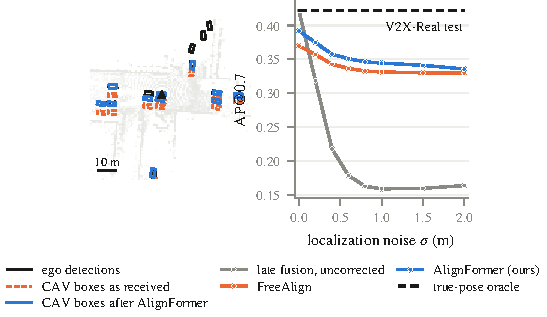
\includegraphics[width=\linewidth]{figures/teaser.pdf}
  \caption{\textbf{Localization error and what remains of it.} Left: a \vxreal frame (val) whose CAV reports its pose with $\sigma=\SI{2}{m}$ noise. Its boxes arrive \SI{4.4}{m} from where the objects are, beside the ego's own detections of the same cars, and late fusion keeps both. \paper puts them \SI{0.11}{m} from the truth from the boxes alone. Right: \ap{0.7} on \vxreal test (2,172 frames, mean of 5 noise seeds, standard errors below the marker size) against the localization noise $\sigma$, whose yaw component is $\sigma$ degrees. Uncorrected late fusion loses 60\% of its clean AP by $\sigma=\SI{1}{m}$. \freealign~\cite{lei2024freealign} recovers most of it, and \paper is above \freealign at every $\sigma$, including $\sigma=0$.}
  \label{fig:teaser}
\end{figure}

Two families of remedies exist. Intermediate-fusion methods~\cite{vadivelu2020learning,lu2023coalign,hong2024mrcnet} correct the pose inside a shared bird's-eye-view feature pipeline. They need megabytes per frame and a jointly trained backbone on every agent. Late-fusion methods work on detected boxes and are therefore cheap and detector-agnostic. The strongest of them, \freealign~\cite{lei2024freealign}, needs no localization at all. It builds a graph per agent whose nodes are boxes and whose edges are relative distances, which are invariant to the sender's pose, matches common subgraphs, and fits the pose by RANSAC over the matched nodes. In our measurements \freealign's correction is flat across the whole noise range, exactly as its paper claims.

\freealign also has two structural weaknesses, and this paper is built on them. First, a relative-distance graph on fewer than three shared objects is degenerate, so \freealign declines the pair. On \opvv it abstains on 84\% of the pairs sharing one or two objects, and on \vxreal those pairs are a quarter of all frames. A method that learns the association from the boxes' absolute geometry, including heading, can answer them. A single matched object with a heading already determines an $\SE$ transform. Second, \freealign's pose is only as good as its hard matches. An exact fit over a wrong correspondence is exactly wrong, and 2.6\% of its corrections on \opvv are off by more than \SI{3}{m}, three times our rate. A soft, learned estimator has the opposite failure. Its answer is a weighted average over candidates, which is never catastrophically wrong but, as the noise grows and the Sinkhorn rows spread over neighbours, is \emph{blurred}. On dense \vxreal pairs at $\sigma=\SI{2}{m}$ its residual is \SI{0.6}{m} against \freealign's \SI{0.3}{m}, and that is where \freealign led.

\paper takes the best of each in a propose-verify-abstain pipeline over the same 7-float boxes \freealign sends (Fig.~\ref{fig:method}). A small transformer over ego and CAV box tokens produces a Sinkhorn soft assignment with dustbins and a closed-form, heading-augmented, inverse-variance-weighted Kabsch pose, refined by two Huber IRLS steps, the \emph{proposal}. An exact re-solve then takes mutually-nearest correspondences under the proposed pose through a shrinking gate schedule and fits $\SE$ by two-point RANSAC over them, the \emph{verification}, which recovers the precision of a hard fit while the learned proposal decides which hypotheses are worth fitting. Finally a Wald test of the proposed correction against its own sandwich covariance, and an agreement rule that accepts the exact fit when it lands within \SI{1}{m} of the proposal or rests on a consensus of at least four hard pairs, decide whether to correct at all, the \emph{abstention}, which is what keeps the clean case from being damaged.

We make four contributions.
\begin{itemize}
  \item A late-fusion aligner over boxes alone whose learned association answers the sparse pairs graph matching cannot (93\% against 16\% coverage, +0.18 against +0.01 \ap{0.7} on those pairs on \opvv), and whose exact verification matches a hard fit's precision on dense pairs (mean residual \SI{0.60}{m} to \SI{0.28}{m} at $\sigma=\SI{2}{m}$).
  \item A calibrated decision to fuse. Nothing in it is learned. The Wald statistic uses the covariance the weighted solve already implies, with a fitted heteroscedastic noise model, and the agreement rule uses the two estimates we already have. Every threshold is selected on validation AP, never on test.
  \item A fair comparison protocol that we believe the field needs. All baselines are re-run under one detector, one evaluator and one paired set of noise draws, each baseline's thresholds selected by its own validation AP, and results reported at three IoU thresholds and by shared-object count. Under this protocol \freealign tuned on mean pose error, the natural criterion for a pose estimator, under-reports itself by 0.061 \ap{0.7} on \vxreal test.
  \item Results on \vxreal and \opvv. \paper leads \freealign at every $\sigma$ and every IoU threshold on \vxreal test, holds under \SIrange{100}{400}{ms} of delay, leads \freealign on \opvv test by 0.009 \ap{0.7} with the same rule, and leads seven intermediate-fusion methods on \opvv from $\sigma=\SI{0.4}{m}$ at $2\times10^4$ to $8\times10^4$ fewer bytes per agent-frame. We also show, with a mechanism, that appearance does not help. Geometry already associates 99.4\% of objects.
\end{itemize}

\section{Related Work}
\label{sec:related}

\input{tables/related_work}

\paragraph{Cooperative perception and its bandwidth.}
V2VNet~\cite{wang2020v2vnet}, OPV2V's AttFuse~\cite{xu2022opv2v}, V2X-ViT~\cite{xu2022v2xvit}, CoBEVT~\cite{xu2022cobevt}, Where2comm~\cite{hu2022where2comm} and F-Cooper~\cite{chen2019fcooper} fuse intermediate BEV features. They set the accuracy ceiling under exact poses and cost megabytes per frame. Late fusion exchanges detected boxes and is the cheapest and most detector-agnostic option. It is also the one whose output depends entirely on the sender's pose being right, which is the problem this paper addresses. Our byte accounting follows OPV2V's convention and charges each method only for what its alignment step adds to the shared box payload.

\paragraph{Pose-error-robust fusion.}
Vadivelu \etal~\cite{vadivelu2020learning} regress a pose correction from fused features and smooth it over the agent graph with a Markov random field. CoAlign~\cite{lu2023coalign} optimises an agent-object pose graph and is the reference robust intermediate method. MRCNet~\cite{hong2024mrcnet} handles pose error and delay together inside the feature pipeline. These need a jointly trained backbone on every agent and the bandwidth that comes with it. On the late-fusion side, RoCo~\cite{huang2024roco} alternates object matching with pose adjustment, and \freealign~\cite{lei2024freealign} removes the pose prior entirely by matching relative-distance graphs and fitting with a robust estimator. \freealign is the comparison that matters for us. It sends the same bytes, needs no localization, and its published ablations put it ahead of CoAlign under large noise. We reimplement it onto our detector and evaluator (Sec.~\ref{sec:protocol}) because its released code is bound to a different detector, postprocessor and AP implementation, and we select its edge threshold on validation AP rather than on pose error, which turns out to matter by 0.06 AP. Fig.~\ref{fig:degenerate} shows why shared-object count affects the two families differently.

\begin{figure}[t]
  \centering
  \resizebox{\linewidth}{!}{\input{figures/degenerate}}
  \caption{\textbf{Why shared-object count matters differently.} A relative-distance graph has one edge over two shared objects, consistent with more than one rotation, and is rigid only from three objects onward. A single shared object with a heading already fixes rotation and translation, so a learned matcher that uses heading can answer pairs a relative-distance graph cannot.}
  \label{fig:degenerate}
\end{figure}

\paragraph{Learned matching and robust registration.}
Our proposal stage is SuperGlue-style~\cite{sarlin2020superglue} attention over two sets with a Sinkhorn~\cite{cuturi2013sinkhorn} assignment and dustbins. The closed-form pose is a weighted Kabsch~\cite{kabsch1976solution} fit. The verification is ICP~\cite{besl1992icp} initialised by the learned estimate with a RANSAC~\cite{fischler1981ransac} inner solve. The robust weighting is Huber IRLS~\cite{huber1964robust}. The abstention is a Wald test~\cite{wald1943tests}. None of these is new. What is new is the composition for this problem, a learned stage that decides \emph{which} correspondences to fit, an exact stage that fits them without blur, and a decision rule that uses the two estimates against each other. We show in Sec.~\ref{sec:ablation} that each stage is worth a measurable amount of AP and that the composition is what overtakes a tuned \freealign.

\paragraph{Asynchrony.}
SyncNet~\cite{lei2022syncnet} and CoBEVFlow~\cite{wei2023cobevflow} compensate communication delay by predicting feature motion. We do not model delay. We measure it, because it is a different error from localization. Static objects arrive correctly placed and moving ones do not, so a rigid correction cannot repair it, and a robust solver must simply not be dragged off by the moving minority. Sec.~\ref{sec:delay} reports both methods under \SIrange{100}{400}{ms}.

\paragraph{Appearance for cross-agent association.}
Re-identification features are the standard cue for associating detections across cameras. We test the hypothesis directly, from colour histograms through frozen ImageNet features to a cross-agent contrastive head on DINOv2~\cite{oquab2023dinov2} patch features, and find it does not move the matcher on either dataset (Sec.~\ref{sec:appearance}). The reason is measurable and we report it.

\section{System Model}
\label{sec:system}

\paragraph{Collaborative perception setting.}
An ego agent and a cooperating agent (CAV) each run their own object detector over their own sensor data and hold a set of locally detected boxes in their own coordinate frame. The CAV transmits its locally detected boxes together with its self-reported pose, its belief about its own position and orientation in the frame the two agents share. The ego agent uses that pose to project the CAV's boxes into its own frame before fusing them with its own detections. We describe one ego-CAV pair. With more than one cooperating agent, the ego agent repeats this for each.

\paragraph{Agent and coordinate frames.}
Each agent's locally detected boxes are expressed in that agent's own sensor frame. The ego agent's detections stay in the ego frame throughout and are written $\mathcal{P}=\{(\mathbf{p}_i,\psi_i,s_i)\}_{i=1}^{M}$. The CAV's locally detected boxes are transformed into the ego frame using the CAV's self-reported pose, giving $\mathcal{Q}=\{(\mathbf{q}_j,\phi_j,s_j)\}_{j=1}^{N}$. $\mathbf{p}_i,\mathbf{q}_j\in\R^2$ are BEV box centres and $\psi_i,\phi_j$ the corresponding headings, both already expressed in the ego frame. $s_i,s_j$ are the detector's confidence scores.

\paragraph{Shared bounding-box representation.}
Each transmitted detection is a box centre, extents and heading, seven floats, together with its detection confidence score. No appearance feature, learned embedding or map is part of the message. A received detection is exactly that seven-float-plus-score tuple, plus the sender's self-reported pose used to place it in the ego frame.

\paragraph{Misalignment model.}
The CAV's self-reported pose differs from its true pose. GNSS and odometry report position and orientation with an error that neither agent knows at inference time. Projecting the CAV's boxes with the reported pose instead of the true one applies the same rigid error to the whole box set at once, since every box of that agent is transformed by the same pose. We model this as an unknown rigid transform $T=(R(\theta),\mathbf{t})\in\SE$ such that $T\mathbf{q}_j$, not $\mathbf{q}_j$, is where the $j$-th object actually is. $T$ is planar. It captures a translation and a yaw error and leaves roll, pitch and height to the detector. Fig.~\ref{fig:misalignment} illustrates $T$ in the shared frame.

\begin{figure}[t]
  \centering
  \resizebox{\linewidth}{!}{\input{figures/system_model}}
  \caption{\textbf{The misalignment transform $T$.} Grey silhouettes are the true object positions. $\mathcal{P}$ (green) is the ego's own detections, placed correctly. $\mathcal{Q}$ (orange) is the CAV's detections as received under its self-reported pose, displaced from every object by the same rigid transform $T$. Both are expressed in the one shared ego frame.}
  \label{fig:misalignment}
\end{figure}

\paragraph{Problem formulation.}
The ego agent observes $\mathcal{P}$ and $\mathcal{Q}$ only. It has no access to the CAV's true pose and no given correspondence between its own and the CAV's detections of the same physical object. The problem is to recover a correction close to $T$ from $\mathcal{P}$ and $\mathcal{Q}$ alone and apply it to $\mathcal{Q}$, so the corrected boxes can be handed to an otherwise unchanged fusion stage together with $\mathcal{P}$. The system is scored by the detection accuracy of the fused output, not by how close the recovered correction is to $T$. Sec.~\ref{sec:protocol} shows why that distinction is not academic.

\section{Method}
\label{sec:method}

\begin{figure*}[t]
  \centering
  % Fig. 2: the propose / verify / abstain pipeline. Drawn in TikZ so it sets in the paper's font.
\resizebox{\textwidth}{!}{%
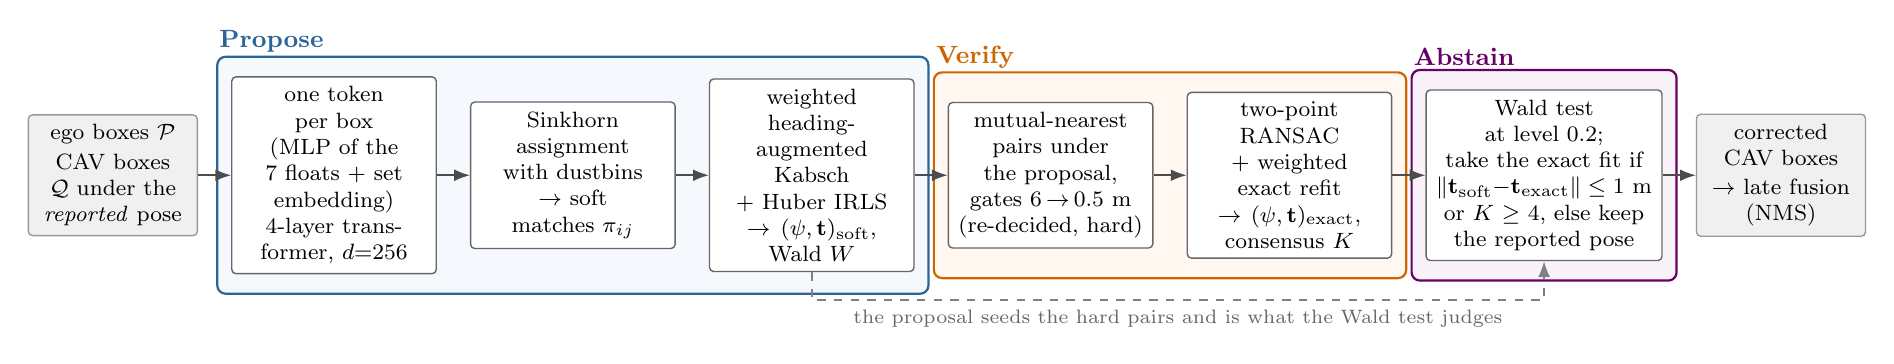
\begin{tikzpicture}[
  >=Latex, node distance=0.42cm,
  blk/.style={draw=black!60, line width=0.5pt, rounded corners=1.5pt, fill=white, inner sep=3.5pt, align=center,
              font=\footnotesize, minimum height=1.25cm, text width=2.35cm},
  io/.style={blk, fill=black!6, draw=black!40, text width=1.9cm},
  stage/.style={draw, rounded corners=3pt, line width=0.8pt, inner xsep=5pt, inner ysep=7pt},
  title/.style={font=\small\bfseries, anchor=south west, inner sep=1pt},
  arr/.style={->, line width=0.6pt, black!70}]
  \node[io] (in) {ego boxes $\mathcal{P}$\\[1pt] CAV boxes $\mathcal{Q}$ under the \emph{reported} pose};
  \node[blk, right=of in] (trunk) {one token per box\\(MLP of the 7 floats + set embedding)\\4-layer transformer, $d{=}256$};
  \node[blk, right=of trunk] (sink) {Sinkhorn assignment with dustbins\\$\to$ soft matches $\pi_{ij}$};
  \node[blk, right=of sink] (kab) {weighted heading-\\augmented Kabsch\\+ Huber IRLS\\$\to(\psi,\mathbf{t})_{\mathrm{soft}}$, Wald $W$};
  \node[blk, right=of kab] (nn) {mutual-nearest pairs under the proposal, gates $6\!\to\!0.5$ m\\(re-decided, hard)};
  \node[blk, right=of nn] (ransac) {two-point RANSAC\\+ weighted exact refit\\$\to(\psi,\mathbf{t})_{\mathrm{exact}}$,\\consensus $K$};
  \node[blk, right=of ransac, text width=2.75cm] (dec) {Wald test at level 0.2;\\take the exact fit if\\$\|\mathbf{t}_{\mathrm{soft}}{-}\mathbf{t}_{\mathrm{exact}}\|\le 1$ m\\or $K\ge 4$, else keep\\the reported pose};
  \node[io, right=of dec] (out) {corrected CAV boxes\\[1pt] $\to$ late fusion (NMS)};
  \foreach \a/\b in {in/trunk, trunk/sink, sink/kab, kab/nn, nn/ransac, ransac/dec, dec/out}
    \draw[arr] (\a) -- (\b);
  \begin{scope}[on background layer]
    \node[stage, draw=cvprblue!80!black, fill=cvprblue!5, fit=(trunk) (kab)] (propose) {};
    \node[stage, draw=orange!80!black, fill=orange!6, fit=(nn) (ransac)] (verify) {};
    \node[stage, draw=violet!80!black, fill=violet!5, fit=(dec)] (abstain) {};
  \end{scope}
  \node[title, text=cvprblue!80!black] at (propose.north west) {Propose};
  \node[title, text=orange!80!black] at (verify.north west) {Verify};
  \node[title, text=violet!80!black] at (abstain.north west) {Abstain};
  \draw[arr, dashed, black!50] (kab.south) -- ++(0,-0.35) -| node[pos=0.25, below, font=\scriptsize, text=black!60] {the proposal seeds the hard pairs and is what the Wald test judges} (dec.south);
\end{tikzpicture}}

  \caption{\textbf{\paper.} The message is the detected boxes. The receiver proposes an $\SE$ correction from a learned soft association, verifies it with an exact fit over the correspondences the proposal implies, and abstains when the two disagree without enough hard evidence. Every stage runs on the 7-float boxes \freealign sends; nothing is added to the message.}
  \label{fig:method}
\end{figure*}

\subsection{Overview}
\label{sec:problem}
\paper estimates the correction $T$ of Sec.~\ref{sec:system} from $\mathcal{P}$ and $\mathcal{Q}$ alone, applies it to the CAV boxes, and hands the corrected set to an unchanged late-fusion stage (per-class NMS over the union). A learned soft association over the box tokens proposes a closed-form pose. An exact re-solve over the correspondences the proposal implies verifies it. A statistical test of the proposal against its own covariance, together with an agreement rule between the two fits, decides whether to abstain. Every design decision below is judged by fused AP, not by pose error; Sec.~\ref{sec:protocol} shows why that distinction is not academic.

\subsection{Propose: learned soft association and closed-form pose}
\label{sec:propose}
\paragraph{Tokens and trunk.}
Each object becomes one token, $\mathrm{MLP}([x,y,z,l,w,h,\cos\psi,\sin\psi,s])$ plus a learned set-membership embedding (ego or CAV). A four-layer transformer ($d=256$, four heads) runs self-attention within each set and cross-attention between them. Object counts are 20 to 60, so this costs nothing measurable. The box carries geometry; nothing else is transmitted (Sec.~\ref{sec:appearance} explains why there is no appearance embedding).

\paragraph{Sinkhorn assignment.}
Trunk outputs are projected to match features, a score matrix $S\in\R^{M\times N}$ is augmented with a dustbin row and column for objects without a counterpart, and 20 Sinkhorn iterations~\cite{cuturi2013sinkhorn} give a soft assignment $P$ with row and column sums bounded by one. For every ego object we form its match mass $w_i=\sum_j P_{ij}$ and virtual counterpart $\hat{\mathbf{q}}_i=\sum_j P_{ij}\mathbf{q}_j/w_i$, with a virtual heading from the mass-weighted heading directions.

\paragraph{Heading-augmented weighted Kabsch.}
Headings enter the same least-squares problem as centres: each object contributes a second virtual point at $\mathbf{p}_i+\lambda\,\mathbf{u}(\psi_i)$ with $\lambda=\SI{2}{m}$, about half a vehicle length, and likewise for $\hat{\mathbf{q}}_i$. Over the augmented, weighted point sets the $\SE$ fit is closed form,
\begin{equation}
\theta=\operatorname{atan2}\!\Big(\textstyle\sum_n w_n\,(\mathbf{q}'_n\!\times\!\mathbf{p}'_n),\ \sum_n w_n\,(\mathbf{q}'_n\!\cdot\!\mathbf{p}'_n)\Big),\quad
\mathbf{t}=\bar{\mathbf{p}}-R(\theta)\bar{\mathbf{q}},
\label{eq:kabsch}
\end{equation}
where primes denote centred points and the sums run over the $2M$ augmented points~\cite{kabsch1976solution}. Yaw is never regressed, which is the structural answer to the yaw collapse that pose-regression heads show on this data (Sec.~\ref{sec:ablation}). Because every matched object contributes a centre and a heading, a single correspondence already determines $\SE$; this is what lets \paper answer pairs sharing one object, where a centre-only or distance-graph method is degenerate.

\paragraph{Inverse-variance weights.}
Least squares is only maximum likelihood when every observation carries the same variance, and here it does not: measured under the \emph{true} pose on held-out data, so that what is measured is detector disagreement and never pose error, the cross-agent centre residual of the same object is \SI{0.53}{m} RMS at the lowest confidence decile and \SI{0.21}{m} at the highest, and the heading residual \ang{13.6} against \ang{3.2}. We fit a two-parameter power law in the pair's minimum score for centre and for heading variance and multiply each correspondence's Sinkhorn mass by the resulting precision. The same model supplies the covariance the abstention test needs (Sec.~\ref{sec:abstain}), so nothing there is fitted twice.

\paragraph{Robust re-weighting.}
Least squares has no redescending influence function: a wrong correspondence with small but non-zero mass biases the fit in proportion to its residual and nothing removes it. Two Huber IRLS~\cite{huber1964robust} steps around Eq.~\eqref{eq:kabsch} ($c=1.345$ on the residual scaled by its predicted standard deviation) down-weight them. The pair falls back to the proposal when the re-weighted evidence drops below three effective objects.

\paragraph{Training.}
Stage~1 trains trunk and match head on the negative log-likelihood of the ground-truth assignment under $P$, dustbins included, with pose noise $\sigma\in[0,\SI{0.5}{m}]$. Stage~2 trains the pose head under a noise curriculum from 0 to \SI{2}{m} on a corner loss: the predicted and the true correction are applied to the CAV boxes and the $L_1$ distance over the four BEV corners is taken, which is in metres throughout, weights heading error by object size automatically and optimises what IoU measures. Ground-truth correspondences come from the datasets' object identities and are used only as supervision; at inference nothing but the boxes is read.

\subsection{Verify: an exact re-solve over the proposed correspondences}
\label{sec:verify}
The proposal's input to Eq.~\eqref{eq:kabsch} is one virtual point per ego object, a mixture of candidates. As pose noise grows the Sinkhorn row spreads over neighbours and the mixture lands between them, so the answer is blurred rather than wrong (Fig.~\ref{fig:residuals}). A hard fit does not blur, and \freealign's advantage on dense pairs is exactly that it decides the correspondence and then fits exactly. We give the proposal the same second step. Starting from $(\theta,\mathbf{t})$, we move the CAV boxes, take the mutually-nearest ego/CAV centre pairs within a gate, fit $\SE$ over them, and repeat with the gate shrinking through $6, 3, 1.5, 0.75, \SI{0.5}{m}$; the schedule's first gate is wide because the proposal can be metres off on the pairs that matter most, and the later gates are what makes the final fit precise. At each stage the fit is not least squares but a two-point RANSAC~\cite{fischler1981ransac} in $\SE$: every pair of correspondences (exhaustively up to 16 pairs, 512 fixed draws beyond) proposes a transform, the transform with the largest consensus at \SI{1}{m} wins, and the heading-augmented exact fit over its inliers is the stage's answer. The number of inliers of the final stage is the fit's \emph{consensus} $c$, which Sec.~\ref{sec:abstain} uses. The step engages when the first gate finds at least three pairs; otherwise the proposal stands. Nothing is learned here and no byte is added.

\subsection{Abstain: a calibrated decision to correct}
\label{sec:abstain}
At low pose error the right action is often no correction, and an estimator that always corrects damages the clean case. Two rules decide, in sequence.

\paragraph{Wald test on the proposal.}
With $A=\sum_n w_n J_n^{\!\top}J_n$ the weighted normal matrix of the solve and $B$ the corresponding sandwich term under the fitted noise model, in which the two augmented points of one object share their centre error (correlation 0.84 at our constants, so treating them as independent would understate the covariance by a factor that is worst exactly where the evidence is thinnest), the covariance of the proposed correction $\hat\vartheta=(\theta,\mathbf{t})$ is $A^{-1}BA^{-1}$ and
\begin{equation}
T^2=\hat\vartheta^{\!\top}\!\big(A^{-1}BA^{-1}\big)^{-1}\hat\vartheta\,/\,\hat\tau^2
\label{eq:wald}
\end{equation}
tests it against ``no correction is needed''~\cite{wald1943tests}, where $\hat\tau^2$ is the one scale the model does not supply, the ratio of observed to predicted weighted residual for that pair. The pair is corrected when $T^2$ exceeds the $\chi^2_3$ quantile at level $\alpha$; $\alpha=0.2$ is selected on validation AP among $\{0.5,0.2,0.1,0.05,0.01\}$ and a per-pair variant.

\paragraph{Agreement with a consensus floor.}
The verified fit replaces the proposal when the two agree, $\lVert\mathbf{t}_{\mathrm{exact}}-\mathbf{t}_{\mathrm{prop}}\rVert\le\SI{1}{m}$, \emph{or} when the exact fit rests on a consensus $c\ge 4$ hard pairs. Without the floor the rule throws away precisely the pairs the verification exists for, those where the proposal is metres off but the exact fit rests on a solid consensus; with it, dense-pair coverage at $\sigma=\SI{2}{m}$ rises from 0.84 to 0.93 at an unchanged \SI{0.25}{m} answered error. If neither condition holds and the Wald test fired, the proposal is used; if the test did not fire, the pair is left uncorrected. Tolerance and floor are selected on validation AP among $\{0.5,1.0\}$~m and $\{0,4,6\}$.

\subsection{What is transmitted}
\label{sec:bytes}
Each agent sends its detected boxes, seven floats and a score, plus its pose: 218 bytes per agent-frame on \vxreal and 439 on \opvv at observed object counts, identical to \freealign. No embedding, feature map or codebook is involved. Earlier versions of this work transmitted a 128-d per-object embedding (8,034 of 8,474 bytes per agent-frame); Sec.~\ref{sec:appearance} reports why it was removed.

\section{Experiments}
\label{sec:experiments}

\subsection{Protocol}
\label{sec:protocol}
\paragraph{Datasets.}
\vxreal~\cite{xiang2024v2xreal} is real traffic with two vehicles and two infrastructure units per scenario; we use the official 48 / 6 / 14 train / val / test scenarios (2,172 test frames, \SI{70}{m} communication range, one vehicle class). \opvv~\cite{xu2022opv2v} is CARLA-simulated V2V traffic; its \texttt{validate} split is a copy of \texttt{test}, so we hold out a scenario-disjoint 15\% of the training scenarios for every selection and report on the official 2,170 test frames. Nothing below is selected on test.

\paragraph{Detector and fusion.}
A PointPillars~\cite{lang2019pointpillars} detector per agent, trained from scratch on each dataset at the full evaluated range, is shared by every method; the fusion stage, NMS over the union of corrected boxes, is also shared. All differences in the tables come from the alignment step alone.

\paragraph{Noise.}
Each CAV pose is perturbed with zero-mean Gaussian noise of standard deviation $\sigma$ metres in $x$ and $y$ and $\sigma$ degrees in yaw, $\sigma\in\{0,0.2,0.4,0.6,0.8,1,1.5,2\}$. Draws are keyed on (seed, $\sigma$, frame, agent), so every method inside one run sees the same perturbed pose and differences between methods are paired; we report five seeds on test and three on validation, and the paired per-seed difference is the statistic. The clean cell is deterministic and run once. Delay is modelled as the CAV transmitting what it saw $d$ frames earlier with its pose at that time, $d\in\{1,2,4\}$ at \SI{10}{Hz}.

\paragraph{Metrics.}
Globally confidence-sorted AP at IoU 0.3, 0.5 and 0.7 over the full test set, per $\sigma$ and as the mean over the sweep. We additionally split frames by the number of ground-truth objects the ego and the CAV share, into 0, 1--2 and 3+, because the two alignment families fail in different buckets. Pose error is reported only as a diagnostic.

\paragraph{Baselines.}
\freealign~\cite{lei2024freealign} is reimplemented onto our detections, sweep and evaluator; its code is bound to a different detector, postprocessor and AP implementation, and running it end to end would not isolate the alignment algorithm. Its six parameters (edge feature, edge threshold, anchor limit, score offset and power, robust estimator) are selected on validation. We found the selection criterion matters: the natural one for a pose estimator, mean pose error, picks a \SI{0.3}{m} edge threshold at which \freealign answers 29\% of \vxreal pairs; selecting the threshold by \freealign's \emph{own validation AP} picks \SI{1.0}{m} (60\% coverage) and is worth +0.061 \ap{0.7} on test. Every \freealign number in this paper is the AP-selected one; the pose-error-selected one is in the supplement. On \opvv we also run seven intermediate-fusion methods under the same sweep: AttFuse~\cite{xu2022opv2v}, V2X-ViT~\cite{xu2022v2xvit}, CoBEVT~\cite{xu2022cobevt}, CoAlign's fusion~\cite{lu2023coalign}, Where2comm~\cite{hu2022where2comm}, F-Cooper~\cite{chen2019fcooper} and V2VAM~\cite{li2023v2vam}, from OpenCOOD checkpoints trained at the same range. The \emph{oracle} corrects every CAV with its true pose and is the ceiling of any aligner; \emph{uncorrected} is late fusion as deployed.

\subsection{Main result on \vxreal}
\label{sec:main}

\begin{table*}[t]
  \centering\small
  \caption{\textbf{\vxreal test, \ap{0.7} against localization noise} (2,172 frames, 5 paired noise seeds; paired standard errors of the sweep-mean differences are $\le 0.0005$). \freealign at its AP-selected threshold. Rows above the rule are the stages of \paper in order; the last is the full method, the one rule selected on validation of both datasets (Sec.~\ref{sec:ablation}). The agreement row is from the RANSAC run; the least-squares row from the earlier run with the same seeds.}
  \label{tab:main}
  \begin{tabular}{l*{8}{c}c}
    \toprule
    $\sigma$ (m / deg) & 0 & 0.2 & 0.4 & 0.6 & 0.8 & 1.0 & 1.5 & 2.0 & mean \\
    \midrule
    uncorrected late fusion & .4223 & .3185 & .2155 & .1771 & .1621 & .1580 & .1584 & .1632 & .2219 \\
    oracle (true pose) & \multicolumn{8}{c}{.4223 at every $\sigma$} & .4223 \\
    \freealign (AP-selected, \SI{1.0}{m}) & .3702 & .3577 & .3420 & .3362 & .3331 & .3321 & .3303 & .3301 & .3415 \\
    \midrule
    propose (Wald $\alpha{=}0.2$) & .3932 & .3404 & .3100 & .3032 & .2993 & .2940 & .2797 & .2661 & .3107 \\
    + verify (ICP, least squares) & .4024 & .3519 & .3269 & .3237 & .3236 & .3239 & .3220 & .3188 & .3366 \\
    + verify (two-point RANSAC, \SI{6}{m} schedule) & \best{.4057} & .3554 & .3288 & .3265 & .3259 & .3265 & .3274 & .3267 & .3404 \\
    + agreement \SI{1.0}{m} & .3902 & .3695 & .3478 & .3413 & .3321 & .3278 & .3149 & .3053 & .3411 \\
    + consensus floor 4 & .3893 & .3721 & .3553 & .3501 & .3456 & .3428 & .3385 & .3349 & .3536 \\
    \textbf{+ weighted refit (\paper)} & .3921 & \best{.3750} & \best{.3576} & \best{.3525} & \best{.3466} & \best{.3445} & \best{.3400} & \best{.3360} & \best{.3555} \\
    \bottomrule
  \end{tabular}
\end{table*}

\begin{table}[t]
  \centering\small
  \caption{\textbf{\vxreal test, sweep means at three IoU thresholds.} Paired standard errors over five seeds.}
  \label{tab:thresholds}
  \resizebox{\linewidth}{!}{\begin{tabular}{lccc}
    \toprule
    & \ap{0.7} & \ap{0.5} & \ap{0.3} \\
    \midrule
    uncorrected & .2219 & .3665 & .4676 \\
    \freealign (AP-selected) & .3415 & .4933 & .5390 \\
    propose & .3107 & .4854 & .5502 \\
    propose + verify (LS) & .3366 & .5038 & .5583 \\
    propose + verify (RANSAC) & .3404 & .5100 & .5642 \\
    propose + verify + agree & .3411 & .5029 & .5537 \\
    + consensus floor & .3536 & \best{.5196} & \best{.5671} \\
    \textbf{\paper} (+ weighted refit) & \best{.3555} & .5185 & .5663 \\
    \quad paired difference to \freealign & $+.0141\pm.0001$ & $+.0255\pm.0002$ & $+.0282\pm.0003$ \\
    \bottomrule
  \end{tabular}}
\end{table}

Table~\ref{tab:main} reads top to bottom as the method was built. The learned proposal alone wins the clean case by 0.023 over \freealign and loses the noisy sweep by 0.031: the soft fit is blurred where \freealign's hard fit is sharp. The exact verification recovers 0.026 of that (paired, $\pm0.0003$) and reverses the order at IoU 0.5 and 0.3. The agreement rule adds 0.004 by declining the pairs where the two estimates disagree. The consensus floor adds 0.012 on the sweep mean, and weighting the exact refit by the soft solve's confidence precisions another 0.002, to a paired lead of $+0.0141\pm0.0001$ over \freealign, ahead at every $\sigma$ including the clean case (.392 against .370) and by 0.006 at \SI{2}{m}; at IoU 0.5 and 0.3 the lead is 0.026 and 0.028 and holds at every $\sigma$ (Table~\ref{tab:thresholds}). The order of the arms on test is the order on validation, where the same rule was +0.0097 and the floor was selected among $\{0,4,6\}$.

\paragraph{Where the two families fail.}
Table~\ref{tab:buckets} splits the test set by shared-object count. On pairs sharing three or more objects (67\% of frames) \freealign's pose-invariant graph is strongest: the plain proposal was 0.10 behind it at $\sigma=\SI{2}{m}$, and the full method is ahead at 0, \SI{0.4}{m} and \SI{1}{m} and 0.003 behind at \SI{2}{m}. On pairs sharing one or two objects (23\%) the graph is degenerate and \freealign is at or below the uncorrected pose, while \paper is 0.04--0.05 above \freealign at every $\sigma>0$. At $\sigma=\SI{2}{m}$ \paper answers 72\% of pairs with a \SI{0.93}{m} mean answered translation error (\SI{0.40}{m} on dense pairs); \freealign answers 60\% at \SI{8.0}{m}, the tail behind its sharp median. With no shared object nothing can be aligned and every method returns the uncorrected pose, which is a check on the evaluator.

\begin{table}[t]
  \centering\small
  \caption{\textbf{\vxreal test \ap{0.7} by shared-object bucket.} Full method in the \paper column.}
  \label{tab:buckets}
  \resizebox{\linewidth}{!}{\begin{tabular}{llcccc}
    \toprule
    bucket (frames) & $\sigma$ & uncorr. & \paper & \freealign & oracle \\
    \midrule
    \multirow{3}{*}{3+ shared (67\%)} & 0 & .437 & .408 & .399 & .437 \\
     & 1.0 & .166 & \best{.400} & .395 & .437 \\
     & 2.0 & .173 & .392 & \best{.395} & .437 \\
    \midrule
    \multirow{3}{*}{1--2 shared (23\%)} & 0 & .426 & .369 & .376 & .426 \\
     & 1.0 & .198 & \best{.252} & .207 & .426 \\
     & 2.0 & .191 & \best{.244} & .200 & .426 \\
    \midrule
    \multirow{2}{*}{0 shared (10\%)} & 0 & .327 & .308 & .327 & .327 \\
     & 2.0 & .214 & .212 & .214 & .327 \\
    \bottomrule
  \end{tabular}}
\end{table}

\begin{table}[t]
  \centering\small
  \caption{\textbf{Association accuracy against localization noise, \vxreal test} (1,696 ego-CAV pairs sharing at least one object, one noise seed). Top-1 over ego objects that have a counterpart; precision / recall of the correspondences each method fits; coverage is the fraction of pairs the method answers. Residual: mean centre error of the corrected CAV boxes, in metres.}
  \label{tab:association}
  \resizebox{\linewidth}{!}{\begin{tabular}{lcc|ccc|ccc}
    \toprule
    & \multicolumn{2}{c|}{Top-1} & \multicolumn{3}{c|}{\paper verified pairs} & \multicolumn{3}{c}{\freealign pairs} \\
    $\sigma$ & nearest & Sinkhorn & P / R & cov. & resid. & P / R & cov. & resid. \\
    \midrule
    0   & 1.000 & .971 & .942 / .828 & .72 & 0.41 & .845 / .825 & .67 & 7.61 \\
    0.4 & 1.000 & .969 & .943 / .828 & .71 & 0.41 & .845 / .825 & .67 & 7.61 \\
    1.0 & .986 & .961 & .941 / .826 & .71 & 0.41 & .845 / .825 & .67 & 7.61 \\
    1.5 & .959 & .943 & .943 / .822 & .71 & 0.47 & .845 / .825 & .67 & 7.61 \\
    2.0 & .913 & .919 & .935 / .807 & .71 & 0.57 & .845 / .825 & .67 & 7.61 \\
    \midrule
    3+ shared, 2.0 & .908 & .914 & .948 / .807 & .99 & 0.54 & .877 / .834 & .92 & 4.84 \\
    1--2 shared, 2.0 & .950 & .958 & .616 / .798 & .15 & 0.97 & .262 / .512 & .18 & 35.3 \\
    \bottomrule
  \end{tabular}}
\end{table}

\paragraph{Association against noise.}
Table~\ref{tab:association} separates the matching from the fitting. \freealign's association is pose-invariant and identical at every $\sigma$: 0.85 precision overall, 0.88 on dense pairs, and 0.26 on the sparse pairs it answers, with a \SI{33}{m} median residual there. Our Sinkhorn Top-1 degrades from 0.971 to 0.919 across the sweep, and is a little below the nearest-centre rule at low noise, but the correspondences behind the verified fit do not degrade: 0.94 precision at every $\sigma$, because the re-solve re-decides them geometrically from the proposed pose, and their residual (\SI{0.41}{m}, median 0.31) is the oracle's on dense pairs. On sparse pairs we engage 15 to 17\% at 0.62 precision where \freealign answers 18\% at 0.26.

\begin{figure}[t]
  \centering
  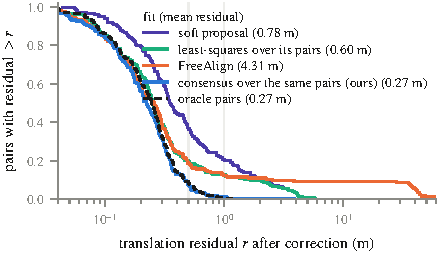
\includegraphics[width=\linewidth]{figures/residuals.pdf}
  \caption{\textbf{Blur, not error.} Fraction of dense \vxreal val pairs ($\sigma=\SI{2}{m}$, 194 pairs) whose translation residual after correction exceeds $r$. The proposal's correspondences are 95\% precise and 98\% complete, yet a least-squares fit over them leaves 13\% of pairs more than \SI{1}{m} off: a few wrong pairs carry full weight. A consensus fit over the \emph{same} pairs is the oracle-correspondence fit (\SI{0.27}{m} mean, 1\% over \SI{1}{m}); \freealign's \SI{0.26}{m} median hides a 12\% tail of wrong answers.}
  \label{fig:residuals}
\end{figure}

\subsection{Communication delay}
\label{sec:delay}
\begin{table}[t]
  \centering\small
  \caption{\textbf{Test under communication delay}, sweep means over $\sigma\in\{0,0.4,1,2\}$, 3 paired seeds; propose+verify+agree is the full method before the consensus floor. Last column: the full method.}
  \label{tab:delay}
  \resizebox{\linewidth}{!}{\begin{tabular}{llcccc}
    \toprule
    delay & metric & oracle & propose+verify+agree & \freealign & \paper \\
    \midrule
    \multicolumn{6}{l}{\textit{\vxreal}} \\
    \multirow{3}{*}{\SI{100}{ms}} & \ap{0.7} & .3421 & .2865 & .2842 & \textbf{.2968} \\
     & \ap{0.5} & .5588 & .4562 & .4428 & \textbf{.4728} \\
     & \ap{0.3} & .6075 & .5349 & .5124 & \textbf{.5509} \\
    \addlinespace
    \multirow{3}{*}{\SI{200}{ms}} & \ap{0.7} & .3189 & .2639 & .2574 & \textbf{.2755} \\
     & \ap{0.5} & .4815 & .4002 & .3846 & \textbf{.4182} \\
     & \ap{0.3} & .5673 & .4818 & .4540 & \textbf{.4982} \\
    \addlinespace
    \multirow{3}{*}{\SI{400}{ms}} & \ap{0.7} & .3136 & .2581 & .2529 & \textbf{.2711} \\
     & \ap{0.5} & .4463 & .3713 & .3604 & \textbf{.3891} \\
     & \ap{0.3} & .4880 & .4277 & .4040 & \textbf{.4433} \\
    \midrule
    \multicolumn{6}{l}{\textit{\opvv}} \\
    \multirow{3}{*}{\SI{100}{ms}} & \ap{0.7} & .3507 & .6383 & .6352 & \textbf{.6425} \\
     & \ap{0.5} & .8546 & .8624 & .8451 & \textbf{.8660} \\
     & \ap{0.3} & .9533 & .9280 & .9037 & \textbf{.9308} \\
    \addlinespace
    \multirow{3}{*}{\SI{200}{ms}} & \ap{0.7} & .2243 & .4976 & .4972 & \textbf{.5064} \\
     & \ap{0.5} & .4072 & .7191 & .7061 & \textbf{.7295} \\
     & \ap{0.3} & .7915 & .8539 & .8235 & \textbf{.8599} \\
    \addlinespace
    \multirow{3}{*}{\SI{400}{ms}} & \ap{0.7} & .2607 & .3873 & .3823 & \textbf{.4020} \\
     & \ap{0.5} & .3427 & .5644 & .5605 & \textbf{.5880} \\
     & \ap{0.3} & .4475 & .6935 & .6629 & \textbf{.7152} \\
    \bottomrule
  \end{tabular}}
\end{table}

Delay is not more localization error: static objects arrive correctly placed and moving ones displaced by their velocity times the delay, so no rigid correction repairs it and a solver must not be dragged off by the moving minority. Table~\ref{tab:delay} shows the ordering of Table~\ref{tab:thresholds} holds under delay on both datasets, at every $\sigma$ and every threshold. On \vxreal the full method leads \freealign by $+0.013$ / $+0.030$ / $+0.039$ \ap{0.7} / \ap{0.5} / \ap{0.3} at \SI{100}{ms} $+0.018$ / $+0.034$ / $+0.044$ at \SI{200}{ms} and $+0.018$ / $+0.029$ / $+0.039$ at \SI{400}{ms} (paired SE $\le 0.0006$): the lead grows from 100 to \SI{200}{ms} and holds at \SI{400}{ms}. On \opvv it leads by $+0.007$ / $+0.021$ / $+0.027$, $+0.009$ / $+0.024$ / $+0.036$ and $+0.020$ / $+0.028$ / $+0.052$ at 100 / 200 / \SI{400}{ms} (SE $\le 0.0006$), at every $\sigma$, and there the lead grows at every step. Huber IRLS down-weights the moving objects; \freealign's relative-distance graph has no equivalent, since one moving object changes its distance to every other node. The verify and agree stages are what make this hold: the per-pair rule of the deployed pipeline, which has neither, was \emph{behind} \freealign at \ap{0.7} under delay on \opvv ($-0.011$ / $-0.032$ / $-0.041$ on the sweep means against the same \freealign), since a fit that follows the moving majority most tightly scores best against a ground truth that does not move with it, and \freealign's fit is tighter than a soft proposal; the consensus fit over verified pairs is tighter still.

\subsection{\opvv: against intermediate fusion and \freealign}
\label{sec:opv2v}
\begin{table*}[t]
  \centering\small
  \caption{\textbf{\opvv test, \ap{0.7} against localization noise}, 2,170 frames, all methods under one detector range, one evaluator and paired noise draws. Intermediate-fusion methods from OpenCOOD checkpoints. Bytes per agent-frame: for intermediate fusion the float32 feature tensor each agent transmits at the fusion site, measured over 100 frames ($^\dagger$Where2comm: \SI{7.3}{MB} after its communication mask, 21\% rate); for the box-only aligners the overhead beyond the shared box payload of \SI{439}{B}, which is zero for both. \paper is the same rule as on \vxreal, selected jointly on both validation sets; 5 paired noise seeds for the box-only aligners.}
  \label{tab:opv2v}
  \begin{tabular}{lr*{8}{c}}
    \toprule
    $\sigma$ (m / deg) & bytes & 0 & 0.2 & 0.4 & 0.6 & 0.8 & 1.0 & 1.5 & 2.0 \\
    \midrule
    uncorrected late fusion & 0 & .8964 & .5978 & .3158 & .2154 & .1844 & .1763 & .1799 & .1898 \\
    F-Cooper~\cite{chen2019fcooper} & \SI{36.0}{MB} & .8402 & .7117 & .4445 & .2858 & .2037 & .1788 & .1506 & .1469 \\
    Where2comm~\cite{hu2022where2comm} & \SI{34.6}{MB}$^\dagger$ & .7849 & .7117 & .5851 & .4695 & .4106 & .3894 & .3851 & .4106 \\
    AttFuse~\cite{xu2022opv2v} & \SI{9.0}{MB} & .8638 & .7758 & .5983 & .5002 & .4648 & .4533 & .4447 & .4481 \\
    CoBEVT~\cite{xu2022cobevt} & \SI{34.6}{MB} & .8773 & .7824 & .5377 & .3807 & .2983 & .2746 & .2538 & .2544 \\
    V2VAM~\cite{li2023v2vam} & \SI{9.0}{MB} & .8975 & .8006 & .5702 & .4109 & .3385 & .3181 & .3410 & .3741 \\
    CoAlign fusion~\cite{lu2023coalign} & \SI{9.0}{MB} & .8831 & .7889 & .6150 & .5324 & .5090 & .5028 & .5023 & .5057 \\
    V2X-ViT~\cite{xu2022v2xvit} & \SI{8.7}{MB} & .8174 & .7894 & .7319 & .6732 & .6250 & .6027 & .5675 & .5515 \\
    \midrule
    \freealign~\cite{lei2024freealign} (pose-error-selected) & 0 & .8461 & .8334 & .8164 & .8094 & .8069 & .8054 & .8048 & .8047 \\
    \freealign (AP-selected, \SI{1.5}{m}) & 0 & .8406 & .8344 & .8236 & .8196 & .8178 & .8175 & .8174 & .8172 \\
    \paper, propose only & 0 & .8674 & .8359 & .8234 & .8185 & .8144 & .8137 & .8109 & .7976 \\
    \textbf{\paper} & 0 & .8526 & \best{.8433} & \best{.8320} & \best{.8282} & \best{.8277} & \best{.8264} & \best{.8262} & \best{.8252} \\
    \bottomrule
  \end{tabular}
\end{table*}
Table~\ref{tab:opv2v} is the comparison the bandwidth argument rests on. Every intermediate-fusion method is above the box-only aligners under exact poses, as it should be with a fused feature map of 8.7 to \SI{36}{MB} per agent-frame against \SI{439}{B} of boxes, and every one collapses from $\sigma=\SI{0.4}{m}$; V2X-ViT degrades most gracefully and is still 0.19 below \paper at \SI{2}{m}. Against \freealign re-selected on its own validation AP (\SI{1.5}{m}; its pose-error selection at \SI{0.5}{m} is 0.004 lower), the full method leads by $+0.0089\pm0.0001$ \ap{0.7} and 0.022 at IoU 0.5 and 0.3 on the sweep means, at every $\sigma$ including the clean case. The two tie on the 80\% of frames sharing three or more objects (.862 against .865 at \SI{2}{m}); the lead is the sparse bucket (13\% of test frames), where \freealign's graph is degenerate: .471 against .352 at \SI{2}{m}. The proposal stage alone, with its per-pair rule, is within 0.001 of \freealign; the weighted exact refit is what makes the difference on this dataset, because \opvv's detections are precise enough that an unweighted hard fit loses to the confidence-weighted soft one (Sec.~\ref{sec:ablation}).

\subsection{Ablations and selection}
\label{sec:ablation}
\begin{table}[t]
  \centering\small
  \caption{\textbf{Selection on \vxreal validation} (3 seeds, sweep-mean \ap{0.7}; paired SE $\le 0.0003$). Every row is one decision made before test.}
  \label{tab:ablation}
  \resizebox{\linewidth}{!}{\begin{tabular}{lcc}
    \toprule
    arm & \ap{0.7} & vs \freealign \\
    \midrule
    \freealign (AP-selected) & .3702 & \\
    propose, Wald 0.2 & .3456 & $-$.0246 \\
    + verify, ICP least squares, gates 2/1/0.5 & .3688 & $-$.0014 \\
    + verify, RANSAC, gates 2/1/0.5 & .3712 & +.0010 \\
    + verify, RANSAC, gates 4/2/1/0.5 & .3725 & +.0023 \\
    + verify, RANSAC, gates 6/3/1.5/0.75/0.5 & .3730 & +.0028 \\
    \quad + candidate search \SI{8}{m} / \SI{12}{m} & .3730 & +.0028 \\
    + agreement \SI{1.0}{m} & .3756 & +.0054 \\
    + agreement \SI{0.5}{m}, floor 4 & .3787 & +.0085 \\
    + agreement \SI{1.0}{m}, floor 6 & .3774 & +.0072 \\
    + agreement \SI{1.0}{m}, floor 4 & .3803 & +.0096 \\
    \quad gated on the Wald decision & .3720 & +.0012 \\
    \textbf{+ weighted exact refit} & \best{.3804} & \best{+.0097} \\
    \quad gated, weighted & .3721 & +.0014 \\
    \midrule
    pose-regression head (no matching) & \multicolumn{2}{c}{collapses to predict-zero} \\
    message + 128-d LiDAR embedding (per-pair arm: .3568 vs .3436 boxes-only) & \multicolumn{2}{c}{+.013 val, $\pm$.001 test} \\
    message + DINOv2 appearance head, verify arm (Sec.~\ref{sec:appearance}) & .3553 & $-$.0135 vs .3688 \\
    \bottomrule
  \end{tabular}}
\end{table}
Table~\ref{tab:ablation} is the record of every choice. The last four rows were selected jointly with \opvv validation under a rule fixed in advance, the largest mean over the two datasets of the paired lead over \freealign: on \opvv the unweighted refit lost 0.012 to \freealign, because its unweighted hard fit is less precise than the confidence-weighted soft one where detections are clean, and the weighted refit recovers 0.010 of that at no cost on \vxreal; gating the agreement rule on the Wald decision helps \opvv by 0.001 and costs \vxreal 0.008, and is not used. Three more things stand out. The hard fit is what matters, not its gate: the three RANSAC schedules are within 0.002 of each other and an explicit search for a better pose basin adds nothing on top of the widest. A direct pose-regression head, the design of the method we started from, never leaves the conditional mean on this data (yaw MAE equal to predicting zero at every $\sigma$), which is why yaw is solved analytically. And the per-object embedding that the message originally carried is within noise of the box-only trunk on both datasets and both splits with no stable sign, at 18 times the bytes; it was removed.

\subsection{Appearance does not help, and why}
\label{sec:appearance}
\begin{table}[t]
  \centering\small
  \caption{\textbf{Cross-agent identity from appearance on \vxreal validation.} AUC of same-object against nearest-neighbour pairs; the bar for a cue to be worth transmitting was 0.80 in both buckets.}
  \label{tab:appearance}
  \resizebox{\linewidth}{!}{\begin{tabular}{lccc}
    \toprule
    cue & dense pairs & sparse pairs & in the matcher \\
    \midrule
    colour histogram & .63 & -- & -- \\
    frozen ImageNet ResNet-18 & .60 & -- & $-$.012 \ap{0.7} \\
    DINOv2-B, zero-shot & .68 & .65 & -- \\
    + contrastive head, GT identities & .85 & .54 & -- \\
    + hard negatives, track pooling & .90 & .885 & $-$.011 \ap{0.7} \\
    + trained on detections & .84 & -- & $-$.011 \ap{0.7} \\
    \bottomrule
  \end{tabular}}
\end{table}
A natural reading of Table~\ref{tab:buckets} is that the sparse bucket needs an appearance cue to disambiguate the one or two shared objects. We tested it to the end. A cross-agent contrastive head on frozen DINOv2 patch features, with the nearest partner-frame vehicles as hard negatives and per-agent track pooling, separates cross-agent identities at AUC 0.885 on sparse pairs, well over the bar we set. Fed into the matcher as a 128-d per-object embedding it moves the sweep mean by $-$0.011 \ap{0.7} (+0.006 in the clean case). The mechanism is in the numbers: stage-1 association is 99.4\% Top-1 correct from geometry alone at the \SI{0.5}{m} noise stage~1 validates at, and Table~\ref{tab:association} shows the verified correspondences at 0.94 precision at every $\sigma$ with the oracle's residual on dense pairs, so there is almost nothing for appearance to fix, and the embedding's cost is pose-displaced tokens that the pose-invariant box geometry does not pay. The remaining gap to the oracle is solver precision on dense pairs, which the verification stage addresses with no new bytes.

\section{Discussion}
\label{sec:discussion}

\paragraph{Why propose, then verify.}
A learned soft matcher and a hard geometric fit fail in opposite ways. The soft fit is never catastrophically wrong, because it averages, and never sharp, for the same reason; the hard fit is sharp when its correspondences are right and exactly wrong when they are not. Using the learned stage to decide \emph{which} correspondences are worth fitting, and the exact stage to fit them, gets the mean of the one and the median of the other. On dense \vxreal pairs at $\sigma=\SI{2}{m}$ the proposal's correspondences are 95\% precise and 98\% complete yet its residual is \SI{0.60}{m}; fitting those same correspondences exactly gives \SI{0.28}{m}, within \SI{0.01}{m} of the fit over oracle correspondences. There was nothing left to learn there; there was something left to solve.

\paragraph{Why abstain, and why not learn it.}
The clean case is the one a deployed system sees most of the time, and every aligner in Table~\ref{tab:main} damages it. The Wald test is the cheapest principled fix: the weighted solve already implies a covariance, the noise model is fitted once on held-out detector disagreement, and the only free quantity is a per-pair residual scale. A learned gate would need labels for ``this correction helped AP'', which do not exist per pair. The consensus floor is the same idea applied to the exact fit: its inlier count is evidence the rule should not discard.

\paragraph{On the size of the margin.}
The lead over an AP-tuned \freealign on the sweep mean is 0.014 \ap{0.7} on \vxreal test and 0.009 on \opvv test, with paired standard errors of 0.0001; on \opvv validation, which is almost entirely dense pairs, the same rule was 0.002 behind. It is small in absolute terms and we do not want to oversell it; the claims we would defend are that the lead is at every $\sigma$, at every IoU threshold, under delay, and at all but the noisiest cell of the bucket where \freealign is structurally strongest, while the clean case is +0.02 and the sparse bucket +0.04 to +0.05. The comparison against a \freealign tuned on pose error, the configuration its paper's protocol implies, would show a 0.07 lead; we report the harder one.

\paragraph{Fair baselines.}
Every number in this paper is a local run under one evaluator; no published number is quoted beside ours, because detector, range, postprocessor and AP implementation differ across codebases by more than the effects measured here. This is a limitation for readers who want to place the absolute numbers, and a strength for the comparisons. The \freealign re-calibration result in Sec.~\ref{sec:protocol} is, we think, a cautionary note for the robust-fusion literature: a pose estimator's natural metric and the detection metric it serves can disagree by more than the differences between methods.

\paragraph{Limitations.}
\paper handles a planar rigid error; roll, pitch and height are left to the detector. It needs at least one shared object with a confident heading, and with none it correctly does nothing, which is 10\% of \vxreal frames. Delay is measured, not modelled, and a motion-aware correction would help the moving minority we currently down-weight. The intermediate-fusion comparison exists on \opvv only, and both datasets are two-agent-pair evaluations; multi-agent consistency through a pose graph was tested and added nothing here because a third agent rarely bridges a sparse pair, but it may on denser deployments.

\section{Conclusion}
\label{sec:conclusion}
We set out to beat the strongest localization-free cooperative aligner at its own bytes and found that the way to do it was not a better matcher but a better division of labour: a learned association to propose, an exact fit to verify, and a calibrated test to abstain. The learned stage answers the sparse pairs where graph matching is degenerate, the exact stage restores the precision a soft estimate blurs on dense pairs, and the decision rule keeps the clean case. On real traffic \paper leads a \freealign tuned on the reported metric at every noise level and IoU threshold and under delay, and on \opvv the same rule leads \freealign and leads intermediate fusion from \SI{0.4}{m} of noise at a thousandth of the bandwidth. Two negative results, that pose-error calibration under-reports a pose estimator by 0.06 AP and that appearance cannot improve an association geometry already gets 99.4\% right, are in our view as useful to the field as the method. Code, the reimplemented baselines, every calibration file and the result JSONs behind every table will be released.

{
    \small
    \bibliographystyle{ieeenat_fullname}
    \bibliography{main}
}
\clearpage
\setcounter{page}{1}
\maketitlesupplementary
\appendix
\setcounter{table}{0}\renewcommand{\thetable}{S\arabic{table}}
\setcounter{figure}{0}\renewcommand{\thefigure}{S\arabic{figure}}

This supplement gives the material the main text points to: the \freealign reimplementation and how its threshold was chosen (\cref{sec:supp_freealign}), the fitted noise model (\cref{sec:supp_variance}), the covariance behind the Wald test and its calibration (\cref{sec:supp_wald}), the per-$\sigma$ and per-seed tables behind every sweep mean (\cref{sec:supp_tables}), the dense-pair diagnosis (\cref{sec:supp_dense}), the appearance probes (\cref{sec:supp_appearance}) and the delay tables (\cref{sec:supp_delay}). Every number is read from a result file in the experiment repository, named in the table captions; nothing in this supplement was selected on test.

\section{\freealign reimplementation and calibration}
\label{sec:supp_freealign}

\paragraph{What is reimplemented.}
\freealign~\cite{lei2024freealign} is ported, not run: the released code is bound to CoAlign's fork of OpenCOOD, an uncertainty-aware detector, g2o and the authors' checkpoints, none of which can be scored under our detector, evaluator and paired noise draws. Every configuration record in our result files carries \texttt{authors\_code\_used: false}. The port follows Section~IV of the paper. Each detected box is a node of a complete graph whose edge attribute is the relative centre distance; a second variant adds the relative yaw, wrapped to $(-\pi,\pi]$ and weighted by $k{=}1$, as the authors' shipped \texttt{greedy\_match.py} does (theirs subtracts raw yaws without wrapping). Matching is their four-step maximum-common-subgraph search: anchor pairs, anchor lists grown by edge discrepancy below the threshold up to $\gamma$ anchors, incremental subgraph growth with greedy ties broken by discrepancy, and selection of the subgraph minimising $(\epsilon_0+\sum_e\epsilon_e)/r^{p}$; with the code's constant $\epsilon_0{=}100$ this prefers the largest subgraph. Fewer than three matched nodes discards the message and the CAV is fused uncorrected. The pose is then fitted by RANSAC or LMedS around an unweighted closed-form $\SE$ solve, enumerating every two-correspondence sample (evenly subsampled above 512), so the fit is deterministic. Not ported: EdgeGAT, the learned edge feature, which the authors' own Table~VI prices at \SI{0.283}{m} against \SI{0.266}{m} without it and whose released configurations switch off; and clock-deviation estimation, which is out of scope.

\paragraph{The grid.}
Six parameters are gridded on validation (\texttt{calibrate\_freealign.py}): edge feature $\{$distance, distance+yaw$\}$, threshold $\{0.3,0.5,1.0,1.5\}$\,m (later widened by $\{0.1,0.15,0.2\}$), $\gamma\in\{1,2,3\}$, $\epsilon_0\in\{0,100\}$, $p\in\{1,3\}$ and estimator $\{$RANSAC, LMedS$\}$: 192 configurations (336 widened), with the minimum node count probed in $\{2,3,4\}$ on the winner. The pose-error criterion is translation MAE over all pairs at $\sigma=\SI{1}{m}$ with an abstention scored as the uncorrected pose, on \opvv's scenario-disjoint validation slice (stride 8, 234 pairs) and \vxreal's official val (stride 4, 245 pairs; a stride-1 re-run on 975 pairs and a run on val plus 44 training scenarios, 4,852 pairs, select the same values). The other five parameters are flat under every criterion; $p$ ties exactly because $\epsilon_0{=}100$ makes the score depend on subgraph size alone.

\paragraph{Pose-error selection against AP selection.}
On \opvv the MAE criterion selects distance, \SI{0.5}{m}, $\gamma{=}3$, $\epsilon_0{=}100$, $p{=}1$, LMedS (MAE \SI{0.099}{m}, coverage 1.0); a yaw channel is three times worse there (\SI{0.290}{m}) because the detector reports a box's axis but not its direction and 20\% of cross-agent detections disagree by $180^\circ$. On \vxreal it selects distance+yaw, \SI{0.3}{m}, $\gamma{=}2$, RANSAC: MAE \SI{1.21}{m} at 29\% coverage. \Cref{tab:supp_fathr} shows why that is the wrong selection for a detection metric: MAE charges nothing for abstaining, so it rewards a threshold and a yaw channel that reject most pairs, and the \SI{0.3}{m} correction that was \SI{0.43}{m} on val grows to \SI{2.68}{m} on test. Selected by its own validation \ap{0.7} sweep mean, \freealign moves to \SI{1.0}{m} on \vxreal (\SI{1.5}{m} is the literal argmax by 0.00005; \SI{1.0}{m} wins \ap{0.5}, \ap{0.3} and the clean case, the tie-break recorded before test was read) and to \SI{1.5}{m} on \opvv. The test difference on \vxreal is $+0.061$ \ap{0.7}. Every \freealign number in the main text is at the AP-selected threshold.

\begin{table}[t]
  \centering\small
  \caption{\textbf{\freealign's edge threshold on validation and test.} \vxreal: val \ap{0.7} sweep mean (3 seeds), $\sigma{=}0$ coverage, and the test sweep mean where it was run; the other parameters are the MAE winner's. \opvv: val MAE at $\sigma{=}\SI{1}{m}$ and val \ap{0.7} sweep mean. Sources: \texttt{freealign\_calibration\_*\_result.json}, \texttt{B\_boxes\_only\_fathr*\_val}, \texttt{B\_boxes\_only\_faap*\_test}, \texttt{fathr*\_val\_result.json}.}
  \label{tab:supp_fathr}
  \resizebox{\linewidth}{!}{%
  \begin{tabular}{lccc|cc}
    \toprule
    & \multicolumn{3}{c|}{\vxreal} & \multicolumn{2}{c}{\opvv} \\
    threshold & val \ap{0.7} & cov. & test \ap{0.7} & val MAE & val \ap{0.7} \\
    \midrule
    \SI{0.1}{m}  & .2582 & .01 & & & \\
    \SI{0.15}{m} & .2660 & .05 & & & \\
    \SI{0.2}{m}  & .2821 & .12 & & & \\
    \SI{0.3}{m} (MAE pick, \vxreal) & .3202 & .27 & .2806 & .373 & .8740 \\
    \SI{0.5}{m} (MAE pick, \opvv)   & .3526 & .40 & & \textbf{.099} & .8959 \\
    \SI{1.0}{m} (AP pick, \vxreal)  & \textbf{.3702} & .56 & \textbf{.3415} & .103 & .8990 \\
    \SI{1.5}{m} (AP pick, \opvv)    & .3703 & .65 & .3393 & .103 & \textbf{.8995} \\
    \bottomrule
  \end{tabular}}
\end{table}

\section{The correspondence variance model}
\label{sec:supp_variance}

\paragraph{Measurement.}
Under the \emph{true} pose on validation ($\sigma{=}0$), so that nothing of the pose enters, every ego detection and CAV detection of the same ground-truth object is a correspondence, and two disagreements are recorded: the centre distance and the heading difference folded to the half-circle (a $180^\circ$ flip is the same axis). \opvv's scenario-disjoint slice gives 6,262 pairs and 63,988 correspondences; \vxreal's val gives 4,334 pairs and 11,652. The overall RMS disagreement is \SI{0.332}{m} and $6.7^\circ$ on \opvv, \SI{0.436}{m} and $10.0^\circ$ on \vxreal. Binned by deciles of the lower of the two detection scores (\cref{tab:supp_deciles}) the RMS falls monotonically with score on both datasets, by a factor of 2.5 in centre and 4.3 in heading on \opvv; the correlation between range and score is $-0.35$ (\opvv) and $-0.14$ (\vxreal), which is why a range term adds nothing once score is in the model.

\begin{table}[t]
  \centering\small
  \caption{\textbf{Cross-agent disagreement by score decile} under the true pose on validation: RMS centre distance (m) and RMS heading difference (deg); first, middle and last decile of $\min(s_{\mathrm{ego}},s_{\mathrm{cav}})$. Sources: \texttt{correspondence\_variance\_result.json} (\opvv), \texttt{variance\_fit\_result.json} (\vxreal).}
  \label{tab:supp_deciles}
  \resizebox{\linewidth}{!}{%
  \begin{tabular}{lcc|cc}
    \toprule
    & \multicolumn{2}{c|}{\opvv} & \multicolumn{2}{c}{\vxreal} \\
    decile (score range) & centre & heading & centre & heading \\
    \midrule
    1 (lowest)  & 0.532 (.20--.28) & 13.6 & 0.503 (.20--.22) & 11.4 \\
    6 (middle)  & 0.281 (.42--.45) & 4.2  & 0.434 (.30--.33) & 9.8 \\
    10 (highest)& 0.214 (.56--.77) & 3.2  & 0.346 (.46--.62) & 5.0 \\
    \bottomrule
  \end{tabular}}
\end{table}

\paragraph{Fitted form.}
Each detection carries a variance that falls as a power of its score, $v(s)=\sigma_1^2\,(s/0.4)^{-2b}$ with the score floored at 0.05 (the detector threshold is 0.2), one pair of constants for the centre and one for the heading. A correspondence's centre variance is the sum of its two detections', $a=v_t(s_{\mathrm{ego}})+v_t(s_{\mathrm{cav}})$, and the variance of its heading point at $\lambda=\SI{2}{m}$ along the axis is $a+\lambda^2\,(v_\psi(s_{\mathrm{ego}})+v_\psi(s_{\mathrm{cav}}))$. The fits are $\sigma_t=\SI{0.2516}{m}$, $b_t=1.128$, $\sigma_\psi=4.64^\circ$, $b_\psi=1.932$ on \opvv and $\sigma_t=\SI{0.2887}{m}$, $b_t=0.493$, $\sigma_\psi=6.01^\circ$, $b_\psi=1.031$ on \vxreal: the real detector is noisier and its score is a weaker predictor, as expected of real traffic. Five forms were compared per channel by the Gamma deviance $\overline{\log v+r^2/v}$ of the squared residual against its modelled variance, the maximum-likelihood criterion for an isotropic Gaussian centre error and a quasi-likelihood for heading (\cref{tab:supp_deviance}); the additive score form was fixed as the selection before the fit. The range form is worth 0.02 on \opvv and nothing on \vxreal; adding range to the score form moves the fitted range scale to $10^{4}$\,m, \ie no range effect. The deployed stage-2 checkpoints use the \emph{scalar} variant of the model, one weight per correspondence from its centre variance applied to both augmented points, which the main text's Eq.~(\ref{eq:kabsch}) describes; the split variant with separate heading weights is available and measured within noise of it.

\begin{table}[t]
  \centering\small
  \caption{\textbf{Noise-model comparison}: Gamma-deviance improvement over the homoscedastic fit, translation / heading (larger is better). Score$_{\min}$ uses the lower score of the pair; additive sums the two detections' variances (selected); $+$range multiplies by $(1+r/r_0)$.}
  \label{tab:supp_deviance}
  \resizebox{\linewidth}{!}{%
  \begin{tabular}{lcc}
    \toprule
    form & \opvv & \vxreal \\
    \midrule
    range $(1+r/r_0)$ & .020 / .020 ($r_0{=}135$ / \SI{119}{m}) & .000 / .000 \\
    score$_{\min}$ & .136 / .457 & .022 / .082 \\
    score additive (selected) & .130 / .438 & .023 / .066 \\
    score additive $+$ range & .130 / .438 ($r_0{=}1.7{\times}10^4$\,m) & .023 / .066 \\
    \bottomrule
  \end{tabular}}
\end{table}

\section{The sandwich covariance of the heading-augmented solve}
\label{sec:supp_wald}

\paragraph{Derivation.}
Write the correction as $\vartheta=(t_x,t_y,\psi)$ and, for each augmented point $n$ (a centre or a heading point $\mathbf{c}+\lambda\,\mathbf{u}(\psi)$ of object $m$) with CAV position $\mathbf{q}_n$, $\mathbf{u}_n=R(\psi)\mathbf{q}_n$ and the Jacobian $J_n=[\,I_2 \mid \mathbf{u}_n^{\perp}\,]$ with $(a,b)^{\perp}=(-b,a)$. The weighted solve has normal matrix $A=\sum_n w_n J_n^{\!\top}J_n$, and its estimator's covariance is $A^{-1}BA^{-1}$ with $B=\sum_{n,n'} w_n w_{n'} J_n^{\!\top}\,\mathrm{Cov}(\epsilon_n,\epsilon_{n'})\,J_{n'}$. The two points of one object are not independent: both carry the object's centre error, so under the fitted model $\mathrm{Cov}(\epsilon_c,\epsilon_c)=\mathrm{Cov}(\epsilon_c,\epsilon_h)=a_m I$ and $\mathrm{Cov}(\epsilon_h,\epsilon_h)=a_m I+\lambda^2 g_m\,\mathbf{d}_m^{\perp}\mathbf{d}_m^{\perp\top}$, where $a_m$ and $g_m$ are the centre and heading variances of \cref{sec:supp_variance} and $\mathbf{d}_m=(\mathbf{u}_h-\mathbf{u}_c)/\lambda$ the unit axis. Collapsing the double sum over the two points of each object,
\begin{align}
B&=\sum_m\Big[\,a_m\,G_m^{\!\top}G_m+\lambda^2 g_m\,w_{h,m}^2\,\mathbf{c}_m\mathbf{c}_m^{\!\top}\Big],\\
G_m&=\big[(w_c{+}w_h)I \mid w_c\mathbf{u}_c^{\perp}+w_h\mathbf{u}_h^{\perp}\big],\quad
\mathbf{c}_m=\big[\mathbf{d}_m^{\perp};\ \mathbf{u}_{h,m}^{\perp}\!\cdot\mathbf{d}_m^{\perp}\big].\nonumber
\end{align}
At the fitted constants and $s{=}0.4$ the correlation between an object's two points is $\sqrt{a/(a+\lambda^2 g)}=0.84$; treating them as independent would understate the covariance by about that factor squared where the evidence is thinnest. One scale the model does not supply is estimated per pair: $\hat\tau^2$ is the weighted residual sum $\sum_n w_n|r_n|^2/v_n$ divided by its expectation under the model (not by a point count), with the weights normalised to the Kish effective count $n_{\mathrm{eff}}=(\sum w)^2/\sum w^2$, and floored so the implied residual standard deviation is at least \SI{0.05}{m}. A relative ridge of $10^{-6}$ is added to $B$ before inversion.

\paragraph{Reference distribution and rules.}
Because $\hat\tau^2$ is estimated, $T^2/p$ is referred to $F(p,D)$ with $p{=}3$ and $D=3\,n_{\mathrm{eff}}-3$ (three noise dimensions per object), whose threshold $p\,F_{1-\alpha}(p,D)$ tends to the $\chi^2_3$ quantile as $D$ grows. Three rules share the statistic: \emph{abstain} zeroes the correction when $T^2$ is below threshold; \emph{per-pair} applies the James--Stein positive part $\max(0,1-p/T^2)$; \emph{both} thresholds and then shrinks. In simulation at nominal 5\% the naive $\sigma^2A^{-1}$ covariance fires on 64\% of null pairs with two matched objects and 27\% with 24; the sandwich fires on 7.5\% and 4.5\%. \Cref{tab:supp_firing} is the empirical check on validation: the fraction of pairs the test corrects at $\sigma{=}0$, where nothing should be corrected, tracks $\alpha$ on both datasets, slightly above it at small $\alpha$ (0.025--0.035 at $\alpha{=}0.01$), and the fraction at $\sigma{=}\SI{2}{m}$ shows what each level gives up. The per-pair rule is close to $\alpha{=}0.5$ in firing rate but shrinks rather than zeroes, which is why it keeps the clean case on \opvv and loses the dense pairs on \vxreal (main text, Sec.~4).

\begin{table}[t]
  \centering\small
  \caption{\textbf{Firing rate of the Wald rule on validation}: fraction of ego--CAV pairs corrected, at $\sigma{=}0$ (the empirical false-fire rate) and at $\sigma{=}\SI{2}{m}$. \vxreal: 975 pairs; \opvv: 1,874 pairs (the 0.1 level was not run there). Sources: \texttt{B\_boxes\_only\_arms\_val\_result.json}, \texttt{abstain\_val\_result.json}.}
  \label{tab:supp_firing}
  \resizebox{\linewidth}{!}{%
  \begin{tabular}{lcc|cc}
    \toprule
    & \multicolumn{2}{c|}{\vxreal} & \multicolumn{2}{c}{\opvv} \\
    rule & $\sigma{=}0$ & $\sigma{=}2$ & $\sigma{=}0$ & $\sigma{=}2$ \\
    \midrule
    abstain, $\alpha{=}0.5$  & .488 & .778 & .512 & 1.000 \\
    abstain, $\alpha{=}0.2$ (selected) & .244 & .686 & .240 & .999 \\
    abstain, $\alpha{=}0.1$  & .156 & .629 & -- & -- \\
    abstain, $\alpha{=}0.05$ & .084 & .591 & .088 & .998 \\
    abstain, $\alpha{=}0.01$ & .025 & .473 & .035 & .996 \\
    per-pair (positive part) & .469 & .776 & .433 & 1.000 \\
    global shrinkage only & .084 & .131 & .222 & .999 \\
    \bottomrule
  \end{tabular}}
\end{table}

\section{Per-sigma tables at IoU 0.5 and 0.3, and per-seed differences}
\label{sec:supp_tables}

\Cref{tab:supp_sigma_v2xreal,tab:supp_sigma_opv2v} give every stage of the method at every sweep $\sigma$ and all three IoU thresholds on both test sets, and \cref{tab:supp_seed_v2xreal,tab:supp_seed_opv2v} the per-seed paired differences to \freealign behind the sweep means quoted in the main text. The five noise seeds are shared by every row, so each column is a comparison on identical draws, and the standard errors of the differences are one to three units in the fourth decimal. The unweighted rows come from the GPU run and the weighted rows from a CPU run of the same seeds; the detector's output differs between devices in the fourth decimal (the uncorrected sweep mean is .2219 against .2225), so each row is compared with the \freealign condition of its own file. The association table of the main text was computed on one noise seed and has no per-seed version; its pooled counts (1,696 pairs) make its precision figures stable to the second decimal.

\begin{table*}[t]
  \centering\small
  \caption{\textbf{V2X-Real test, per-$\sigma$ AP at IoU 0.7, 0.5 and 0.3}, mean over the paired noise seeds of each row's result file. Rows above the rule are references; below it the stages of AlignFormer in order.}
  \label{tab:supp_sigma_v2xreal}
  \begin{tabular}{lccccccccc}
    \toprule
    \multicolumn{10}{l}{\textbf{AP@0.7}} \\
    $\sigma$ (m / deg) & 0 & 0.2 & 0.4 & 0.6 & 0.8 & 1 & 1.5 & 2 & mean \\
    \midrule
    uncorrected late fusion & .4224 & .3182 & .2177 & .1782 & .1623 & .1585 & .1594 & .1633 & .2225 \\
    oracle (true pose) & .4224 & .4224 & .4224 & .4224 & .4224 & .4224 & .4224 & .4224 & .4224 \\
    FreeAlign (AP-selected, 1.0 m) & .3698 & .3572 & .3427 & .3366 & .3327 & .3314 & .3300 & .3300 & .3413 \\
    \midrule
    propose (Wald 0.2) & .3931 & .3419 & .3106 & .3018 & .2987 & .2947 & .2816 & .2636 & .3107 \\
    + verify, least squares & .4024 & .3534 & .3272 & .3223 & .3220 & .3231 & .3230 & .3171 & .3363 \\
    + verify, two-point RANSAC & .4057 & .3563 & .3299 & .3250 & .3247 & .3267 & .3276 & .3268 & .3403 \\
    + agreement 1.0 m & .3902 & .3699 & .3482 & .3380 & .3315 & .3275 & .3186 & .3034 & .3409 \\
    + consensus floor 4 & .3893 & .3723 & .3557 & .3487 & .3449 & .3428 & .3398 & .3339 & .3534 \\
    + weighted refit (AlignFormer) & .3921 & .3747 & .3576 & .3509 & .3464 & .3445 & .3412 & .3357 & .3554 \\
    \addlinespace
    \multicolumn{10}{l}{\textbf{AP@0.5}} \\
    $\sigma$ (m / deg) & 0 & 0.2 & 0.4 & 0.6 & 0.8 & 1 & 1.5 & 2 & mean \\
    \midrule
    uncorrected late fusion & .5942 & .5635 & .4463 & .3430 & .2856 & .2560 & .2263 & .2197 & .3668 \\
    oracle (true pose) & .5942 & .5942 & .5942 & .5942 & .5942 & .5942 & .5942 & .5942 & .5942 \\
    FreeAlign (AP-selected, 1.0 m) & .5272 & .5232 & .5083 & .4937 & .4818 & .4761 & .4684 & .4654 & .4930 \\
    \midrule
    propose (Wald 0.2) & .5584 & .5429 & .5104 & .4874 & .4727 & .4625 & .4400 & .4115 & .4857 \\
    + verify, least squares & .5647 & .5514 & .5209 & .4997 & .4871 & .4803 & .4694 & .4551 & .5036 \\
    + verify, two-point RANSAC & .5706 & .5562 & .5253 & .5037 & .4906 & .4854 & .4758 & .4705 & .5098 \\
    + agreement 1.0 m & .5628 & .5566 & .5329 & .5100 & .4930 & .4811 & .4578 & .4296 & .5030 \\
    + consensus floor 4 & .5613 & .5560 & .5377 & .5208 & .5096 & .5022 & .4907 & .4775 & .5195 \\
    + weighted refit (AlignFormer) & .5608 & .5554 & .5367 & .5205 & .5079 & .5010 & .4890 & .4767 & .5185 \\
    \addlinespace
    \multicolumn{10}{l}{\textbf{AP@0.3}} \\
    $\sigma$ (m / deg) & 0 & 0.2 & 0.4 & 0.6 & 0.8 & 1 & 1.5 & 2 & mean \\
    \midrule
    uncorrected late fusion & .6099 & .6082 & .5846 & .5145 & .4426 & .3854 & .3071 & .2771 & .4662 \\
    oracle (true pose) & .6099 & .6099 & .6099 & .6099 & .6099 & .6099 & .6099 & .6099 & .6099 \\
    FreeAlign (AP-selected, 1.0 m) & .5600 & .5597 & .5572 & .5484 & .5368 & .5272 & .5128 & .5044 & .5383 \\
    \midrule
    propose (Wald 0.2) & .5868 & .5857 & .5801 & .5653 & .5511 & .5347 & .5103 & .4816 & .5494 \\
    + verify, least squares & .5907 & .5901 & .5846 & .5712 & .5570 & .5431 & .5231 & .5033 & .5579 \\
    + verify, two-point RANSAC & .5960 & .5946 & .5893 & .5750 & .5605 & .5481 & .5293 & .5173 & .5638 \\
    + agreement 1.0 m & .5943 & .5936 & .5896 & .5746 & .5574 & .5401 & .5082 & .4729 & .5538 \\
    + consensus floor 4 & .5938 & .5931 & .5901 & .5786 & .5667 & .5557 & .5378 & .5198 & .5670 \\
    + weighted refit (AlignFormer) & .5934 & .5928 & .5896 & .5785 & .5662 & .5551 & .5368 & .5197 & .5665 \\
    \addlinespace
    \bottomrule
  \end{tabular}
\end{table*}

\begin{table*}[t]
  \centering\small
  \caption{\textbf{OPV2V test, per-$\sigma$ AP at IoU 0.7, 0.5 and 0.3}, mean over the paired noise seeds of each row's result file. Rows above the rule are references; below it the stages of AlignFormer in order.}
  \label{tab:supp_sigma_opv2v}
  \begin{tabular}{lccccccccc}
    \toprule
    \multicolumn{10}{l}{\textbf{AP@0.7}} \\
    $\sigma$ (m / deg) & 0 & 0.2 & 0.4 & 0.6 & 0.8 & 1 & 1.5 & 2 & mean \\
    \midrule
    uncorrected late fusion & .8964 & .6183 & .3155 & .2164 & .1842 & .1746 & .1805 & .1897 & .3469 \\
    oracle (true pose) & .8964 & .8964 & .8964 & .8964 & .8964 & .8964 & .8964 & .8964 & .8964 \\
    FreeAlign (AP-selected, 1.5 m) & .8406 & .8346 & .8242 & .8203 & .8180 & .8172 & .8172 & .8173 & .8237 \\
    \midrule
    per-pair rule (deployed before) & .8674 & .8385 & .8230 & .8193 & .8148 & .8131 & .8098 & .7990 & .8231 \\
    propose (Wald 0.2) & .8594 & .8326 & .8176 & .8154 & .8140 & .8118 & .8094 & .7995 & .8200 \\
    + verify, RANSAC, weighted refit & .8756 & .8437 & .8279 & .8263 & .8258 & .8252 & .8250 & .8244 & .8342 \\
    + agreement 1.0 m & .8540 & .8441 & .8302 & .8259 & .8230 & .8215 & .8204 & .8142 & .8292 \\
    + consensus floor 4 (AlignFormer) & .8526 & .8439 & .8322 & .8291 & .8270 & .8261 & .8256 & .8242 & .8326 \\
    per-pair rule + weighted re-solve (not pre-registered) & .8807 & .8502 & .8326 & .8292 & .8265 & .8265 & .8256 & .8230 & .8368 \\
    \addlinespace
    \multicolumn{10}{l}{\textbf{AP@0.5}} \\
    $\sigma$ (m / deg) & 0 & 0.2 & 0.4 & 0.6 & 0.8 & 1 & 1.5 & 2 & mean \\
    \midrule
    uncorrected late fusion & .9503 & .9269 & .6884 & .4692 & .3574 & .3041 & .2584 & .2521 & .5258 \\
    oracle (true pose) & .9503 & .9503 & .9503 & .9503 & .9503 & .9503 & .9503 & .9503 & .9503 \\
    FreeAlign (AP-selected, 1.5 m) & .9176 & .9168 & .9111 & .9040 & .8995 & .8972 & .8941 & .8933 & .9042 \\
    \midrule
    per-pair rule (deployed before) & .9408 & .9374 & .9301 & .9227 & .9174 & .9152 & .9095 & .9006 & .9217 \\
    propose (Wald 0.2) & .9407 & .9376 & .9287 & .9208 & .9166 & .9137 & .9082 & .9002 & .9208 \\
    + verify, RANSAC, weighted refit & .9453 & .9427 & .9329 & .9258 & .9219 & .9192 & .9160 & .9142 & .9273 \\
    + agreement 1.0 m & .9416 & .9407 & .9323 & .9242 & .9184 & .9148 & .9110 & .9028 & .9232 \\
    + consensus floor 4 (AlignFormer) & .9405 & .9396 & .9321 & .9262 & .9217 & .9185 & .9158 & .9132 & .9260 \\
    per-pair rule + weighted re-solve (not pre-registered) & .9433 & .9402 & .9332 & .9271 & .9221 & .9205 & .9172 & .9140 & .9272 \\
    \addlinespace
    \multicolumn{10}{l}{\textbf{AP@0.3}} \\
    $\sigma$ (m / deg) & 0 & 0.2 & 0.4 & 0.6 & 0.8 & 1 & 1.5 & 2 & mean \\
    \midrule
    uncorrected late fusion & .9552 & .9543 & .9149 & .7786 & .6370 & .5403 & .4012 & .3499 & .6914 \\
    oracle (true pose) & .9552 & .9552 & .9552 & .9552 & .9552 & .9552 & .9552 & .9552 & .9552 \\
    FreeAlign (AP-selected, 1.5 m) & .9268 & .9267 & .9259 & .9222 & .9180 & .9146 & .9086 & .9062 & .9186 \\
    \midrule
    per-pair rule (deployed before) & .9509 & .9497 & .9477 & .9446 & .9399 & .9366 & .9316 & .9235 & .9406 \\
    propose (Wald 0.2) & .9518 & .9510 & .9486 & .9444 & .9402 & .9362 & .9306 & .9231 & .9407 \\
    + verify, RANSAC, weighted refit & .9518 & .9508 & .9480 & .9442 & .9403 & .9366 & .9312 & .9277 & .9413 \\
    + agreement 1.0 m & .9497 & .9496 & .9475 & .9438 & .9376 & .9335 & .9270 & .9175 & .9383 \\
    + consensus floor 4 (AlignFormer) & .9490 & .9488 & .9470 & .9439 & .9395 & .9357 & .9305 & .9264 & .9401 \\
    per-pair rule + weighted re-solve (not pre-registered) & .9510 & .9496 & .9472 & .9445 & .9397 & .9371 & .9325 & .9280 & .9412 \\
    \addlinespace
    \bottomrule
  \end{tabular}
\end{table*}

\begin{table*}[t]
  \centering\small
  \caption{\textbf{V2X-Real test, per-seed paired differences to FreeAlign} of the sweep-mean AP: one column per noise seed at IoU 0.7, then mean $\pm$ standard error at the three thresholds. Every row is compared with the FreeAlign condition of its own result file, on identical noise draws.}
  \label{tab:supp_seed_v2xreal}
  \resizebox{\textwidth}{!}{\begin{tabular}{lcccccccc}
    \toprule
    row & seed 0 & seed 1 & seed 2 & seed 3 & seed 4 & AP@0.7 & AP@0.5 & AP@0.3 \\
    \midrule
    uncorrected late fusion & $-$.1194 & $-$.1187 & $-$.1181 & $-$.1193 & $-$.1185 & $-.1188\pm.0002$ & $-.1262\pm.0004$ & $-.0722\pm.0005$ \\
    oracle (true pose) & +.0810 & +.0807 & +.0814 & +.0811 & +.0811 & $+.0811\pm.0001$ & $+.1012\pm.0001$ & $+.0715\pm.0001$ \\
    propose (Wald 0.2) & $-$.0305 & $-$.0304 & $-$.0295 & $-$.0311 & $-$.0313 & $-.0306\pm.0003$ & $-.0073\pm.0005$ & $+.0111\pm.0003$ \\
    + verify, least squares & $-$.0048 & $-$.0060 & $-$.0042 & $-$.0050 & $-$.0056 & $-.0051\pm.0003$ & $+.0103\pm.0005$ & $+.0194\pm.0004$ \\
    + verify, two-point RANSAC & $-$.0011 & $-$.0017 & $-$.0003 & $-$.0010 & $-$.0012 & $-.0011\pm.0002$ & $+.0165\pm.0004$ & $+.0252\pm.0003$ \\
    + agreement 1.0 m & $-$.0003 & $-$.0010 & +.0002 & $-$.0008 & $-$.0006 & $-.0005\pm.0002$ & $+.0097\pm.0003$ & $+.0153\pm.0003$ \\
    + consensus floor 4 & +.0121 & +.0117 & +.0123 & +.0120 & +.0119 & $+.0120\pm.0001$ & $+.0262\pm.0002$ & $+.0284\pm.0003$ \\
    + weighted refit (AlignFormer) & +.0142 & +.0138 & +.0143 & +.0140 & +.0141 & $+.0141\pm.0001$ & $+.0255\pm.0002$ & $+.0282\pm.0003$ \\
    \bottomrule
  \end{tabular}}
\end{table*}

\begin{table*}[t]
  \centering\small
  \caption{\textbf{OPV2V test, per-seed paired differences to FreeAlign} of the sweep-mean AP: one column per noise seed at IoU 0.7, then mean $\pm$ standard error at the three thresholds. Every row is compared with the FreeAlign condition of its own result file, on identical noise draws.}
  \label{tab:supp_seed_opv2v}
  \resizebox{\textwidth}{!}{\begin{tabular}{lcccccccc}
    \toprule
    row & seed 0 & seed 1 & seed 2 & seed 3 & seed 4 & AP@0.7 & AP@0.5 & AP@0.3 \\
    \midrule
    uncorrected late fusion & $-$.4790 & $-$.4768 & $-$.4769 & $-$.4753 & $-$.4754 & $-.4767\pm.0007$ & $-.3784\pm.0007$ & $-.2272\pm.0012$ \\
    oracle (true pose) & +.0729 & +.0726 & +.0729 & +.0728 & +.0725 & $+.0727\pm.0001$ & $+.0461\pm.0001$ & $+.0366\pm.0001$ \\
    per-pair rule (deployed before) & $-$.0008 & $-$.0002 & $-$.0006 & $-$.0003 & $-$.0008 & $-.0006\pm.0001$ & $+.0175\pm.0001$ & $+.0220\pm.0001$ \\
    propose (Wald 0.2) & $-$.0043 & $-$.0031 & $-$.0037 & $-$.0035 & $-$.0037 & $-.0037\pm.0002$ & $+.0166\pm.0001$ & $+.0221\pm.0002$ \\
    + verify, RANSAC, weighted refit & +.0103 & +.0105 & +.0106 & +.0108 & +.0107 & $+.0106\pm.0001$ & $+.0231\pm.0001$ & $+.0227\pm.0002$ \\
    + agreement 1.0 m & +.0057 & +.0054 & +.0054 & +.0053 & +.0056 & $+.0055\pm.0001$ & $+.0190\pm.0001$ & $+.0197\pm.0002$ \\
    + consensus floor 4 (AlignFormer) & +.0092 & +.0091 & +.0088 & +.0087 & +.0088 & $+.0089\pm.0001$ & $+.0218\pm.0001$ & $+.0215\pm.0002$ \\
    per-pair rule + weighted re-solve (not pre-registered) & +.0129 & +.0130 & +.0135 & +.0133 & +.0130 & $+.0131\pm.0001$ & $+.0230\pm.0001$ & $+.0226\pm.0001$ \\
    \bottomrule
  \end{tabular}}
\end{table*}


\section{Dense-pair diagnosis}
\label{sec:supp_dense}

The diagnosis of Sec.~4 of the main text runs every solve variant on the \vxreal val pairs sharing at least three objects (194 pairs at stride 3, one noise seed) and records the translation residual of the corrected CAV boxes against the boxes under the true pose. \Cref{tab:supp_stages} gives the correspondences the re-solve decides at each gate, scored against the ground-truth identities, and \cref{tab:supp_residuals} the residual of each fit. Three facts carry the argument. First, the correspondences are right: 95\% precision and 98\% recall at the first gate, pooled over pairs, where \freealign's graph matching is 87\% precise and 82\% complete on the same pairs and answers 89\% of them. Second, the least-squares fit over those correspondences has a \SI{0.60}{m} mean residual with 13\% of pairs more than \SI{1}{m} off, while the same fit over only the correct pairs is \SI{0.28}{m} and a RANSAC fit over all of the re-solve's pairs \SI{0.27}{m}: the few wrong pairs, with full weight, are the residual. Third, 19 of the 194 pairs never engaged the re-solve because the first \SI{2}{m} gate found fewer than three pairs under a proposal that was \SI{3.4}{m} off on average; a candidate search around the proposal engaged all 19 at \SI{0.23}{m}, and so does the wider \SI{6}{m} gate schedule the method ships, which is why the search is not part of it (val \ap{0.7} .3724 against .3730). At $\sigma=\SI{0.8}{m}$ the same quantities are closer together (proposal \SI{0.39}{m}, least-squares re-solve \SI{0.30}{m}, oracle \SI{0.27}{m}); the gap opens with noise, as the mixture argument of the main text predicts.

\begin{table}[t]
  \centering\small
  \caption{\textbf{Correspondences of the re-solve by gate}, dense \vxreal val pairs at $\sigma{=}\SI{2}{m}$: precision pooled over pairs, mean recall, mean pairs per stage; \freealign's matching on the same pairs. Source: \texttt{dense\_resolve\_diagnosis\_val\_result.json}.}
  \label{tab:supp_stages}
  \resizebox{\linewidth}{!}{%
  \begin{tabular}{lccc}
    \toprule
    stage & precision & recall & pairs \\
    \midrule
    gate \SI{2.0}{m} & .947 & .980 & 5.35 \\
    gate \SI{1.0}{m} & .955 & .986 & 5.37 \\
    gate \SI{0.5}{m} & .963 & .935 & 5.13 \\
    \freealign (answered 172 / 194) & .871 & .818 & -- \\
    \bottomrule
  \end{tabular}}
\end{table}

\begin{table}[t]
  \centering\small
  \caption{\textbf{Translation residual of every fit} on the 194 dense \vxreal val pairs at $\sigma{=}\SI{2}{m}$: pairs answered, median and mean (m), fraction over 0.5 and \SI{1}{m}. Sources: \texttt{dense\_resolve\_diagnosis\_*\_val\_result.json}.}
  \label{tab:supp_residuals}
  \resizebox{\linewidth}{!}{%
  \begin{tabular}{lccccc}
    \toprule
    fit & $n$ & median & mean & $>$0.5 & $>$1 \\
    \midrule
    uncorrected & 194 & 2.60 & 2.67 & .98 & .90 \\
    soft proposal (Huber IRLS) & 194 & 0.35 & 0.78 & .37 & .21 \\
    least-squares re-solve, gates 2/1/0.5 & 194 & 0.25 & 0.60 & .20 & .13 \\
    \quad same, correct pairs only & 174 & 0.25 & 0.28 & .11 & .02 \\
    \quad RANSAC over the same pairs & 175 & 0.22 & 0.27 & .07 & .01 \\
    RANSAC re-solve as shipped (gates 2/1/0.5) & 194 & 0.25 & 0.59 & .19 & .12 \\
    \quad with the \SI{8}{m} candidate search & 194 & 0.24 & 0.28 & .10 & .02 \\
    \freealign & 172 & 0.26 & 4.31 & .19 & .12 \\
    \quad exact fit over \freealign's pairs & 172 & 0.26 & 4.20 & .26 & .17 \\
    oracle correspondences, exact & 194 & 0.24 & 0.27 & .09 & .01 \\
    oracle correspondences, RANSAC & 194 & 0.24 & 0.24 & .04 & .01 \\
    \bottomrule
  \end{tabular}}
\end{table}

\section{Appearance probes}
\label{sec:supp_appearance}

\paragraph{Separability probe.}
For every object two agents both detect at one timestamp, the probe compares the cosine similarity of the ego's crop to its true partner's crop in the CAV against the ego's crop to the CAV's nearest \emph{other} vehicle, and reports the paired AUC. The \emph{ambiguous} subset is the objects with a competitor within \SI{8}{m}, the radius the LiDAR probe used. Crops need at least 50 pixels and at most 0.5 occlusion, and the least-occluded camera is kept; coverage is the fraction of shared objects with a usable crop in both agents, reported overall and by range (0--25, 25--40, 40--70, 70+\,m). Two controls bound the number: a shuffled-identity run must land within 0.02 of 0.5 or the run is void, and a \emph{same-agent} bound compares two cameras of one agent at the same instant, the best any cross-agent cue could do. Three bars were fixed before the first run: ambiguous AUC $\ge 0.80$, coverage $\ge 0.40$, and 40--\SI{70}{m} coverage $\ge 0.25$. Descriptors: a 24$\times$8 hue--saturation histogram over the silhouette mask with the value channel dropped, the mean colour, and on \vxreal frozen DINOv2 (ViT-S/14 and ViT-B/14, 224-px letterboxed crop with 10\% context, class token or silhouette-masked patch mean). \Cref{tab:supp_probe} has the results. On \opvv colour reaches 0.64 (same-agent bound 0.71) at 39\% coverage and fails all three bars; the LiDAR appearance embedding of the detector is 0.63 on the same subset, and its effect on association on the hard subset ($r{=}\SI{5}{m}$, 17,484 objects, $\sigma{=}0.5$) is $+0.0001$ Top-1 with 95\% CI $[-0.0013, +0.0014]$. Three structural reasons were established: the CARLA asset library gives every CAV box a width of $2.014\pm0.081$\,m with competitors differing by a median \SI{0.07}{m}; the \SI{0.8}{m} BEV cell samples a car with about a dozen cells, enough for a size class and not an identity; and there is no ambiguity to resolve, since no ego object in the val split has a competitor within \SI{2}{m} and nearest-centre association is 1.000 Top-1 at $\sigma{=}0$. Under-training was ruled out: the embedding head's weight norm doubles over training, a causal shuffle of the embedding costs the model 0.0036 (it is used), and a retrained boxes-only trunk recovers all of it from geometry. On \vxreal coverage passes (47\%, 36\% at 40--\SI{70}{m}) but the signal fails: colour 0.63, and the same-agent bound is \emph{below} the cross-agent number (0.42 / 0.56), which says the cue is dominated by the camera and its exposure, not the object. Zero-shot DINOv2 reaches 0.68 with bounds of 0.61--0.73.

\begin{table}[t]
  \centering\small
  \caption{\textbf{Appearance separability}, paired AUC of true partner against nearest competitor on the ambiguous subset, with the same-agent bound and coverage. Bars: AUC $\ge$.80, coverage $\ge$.40. Sources: \texttt{camera\_separability\_result.json}, \texttt{colour\_separability\_val\_result.json}, \texttt{appearance\_separability\_*\_val\_result.json}, \texttt{appearance\_head\_*\_val\_result.json}.}
  \label{tab:supp_probe}
  \resizebox{\linewidth}{!}{%
  \begin{tabular}{llccc}
    \toprule
    dataset & descriptor & AUC & same-agent & coverage \\
    \midrule
    \opvv & hue--saturation & .598 & .707 & .39 \\
    \opvv & mean colour & .640 & .680 & .39 \\
    \opvv & LiDAR embedding (detector) & .627 & -- & 1.0 \\
    \vxreal & hue--saturation & .632 & .421 & .47 \\
    \vxreal & mean colour & .612 & .558 & .47 \\
    \vxreal & DINOv2 ViT-S/14, patch mean & .653 & .611 & .47 \\
    \vxreal & DINOv2 ViT-B/14, patch mean & .681 & .653 & .47 \\
    \vxreal & DINOv2 ViT-B/14, class token & .645 & .726 & .47 \\
    \vxreal & trained head, annotations (sparse bucket) & \textbf{.885} & -- & .47 \\
    \vxreal & trained head, detections & .835 & -- & .47 \\
    \bottomrule
  \end{tabular}}
\end{table}

\paragraph{Trained cross-view head.}
To give appearance its best case on real data we trained a head on \vxreal: dropout, linear $1536\!\to\!512$, GELU, dropout, linear $512\!\to\!128$, unit-normalised, over frozen ViT-B/14 descriptors (class token concatenated with the masked patch mean), with a symmetric InfoNCE loss at temperature 0.07 whose positives are the same annotated vehicle in two agents' frames and whose hard negatives are the eight nearest in-frame vehicles of the partner, in-batch false negatives masked by identity. A first head trained for 20 fixed epochs on every second training frame (11,509 agent-frames, 76,330 pairs) reaches 0.845 on all val pairs but 0.537 on the sparse bucket (pairs sharing one or two objects, $n{=}374$) and 1.000 on its own training probe: it memorises. The head reported in the main text holds out the last fifth of training scenarios whole, selects its epoch on held-out far-range AUC (epoch 3), pools each agent's descriptors over its own track with a window of 2 steps (\SI{0.2}{s} each) fixed in advance, and reads val once: 0.885 on the sparse bucket, 0.900 on dense pairs, 0.897 at 40--\SI{70}{m}, 0.838 beyond. Adding colour to its input hurts (0.463; 0.679 with the window). The window matters for the trained head and for nothing else: 0.807 / 0.882 / 0.885 / 0.904 / 0.906 at 0--4 steps on the sparse bucket, flat for zero-shot features and for the memorising head. Trained on annotations it scores only 0.73 on detector boxes; a head trained on the detections themselves reaches 0.835 (0.803 at 40--\SI{70}{m}), on a sparse bucket that shrinks to nine ambiguous objects.

\paragraph{In the matcher.}
Each head's similarity enters the Sinkhorn cost beside the geometric token affinity, with the descriptors pooled causally over up to four earlier frames (\vxreal val, 3 seeds, \ap{0.7}; sources \texttt{B\_dino\{,\_det\}\_icp\_val\_result.json}). With the re-solve arm the sweep mean falls from .3688 to .3553 (annotation head) and .3577 (detection head), paired differences $-0.012$ and $-0.011\pm0.000$; with the agreement rule $-0.003$; for the soft Wald arm $-0.028$ to $-0.030$. The clean case gains $+0.006$ to $+0.009$ and the sparse bucket at $\sigma{=}0$ gains .200 $\to$ .25 on 39 frames. The stage-1 Top-1 on val is .994 with boxes alone and .970 / .976 with a head: under any localization noise from $\sigma{=}0.2$ up the cue makes the soft association \emph{worse} by 0.02--0.03, because a similarity that is right 88\% of the time is noise on the 99\% of pairs geometry already decides. The cue is not shipped.

\section{Communication delay, per sigma}
\label{sec:supp_delay}

\paragraph{Protocol.}
Delay uses OpenCOOD's asynchrony in its deterministic setting (a constant delay, so the paired seeds stay paired; OpenCOOD's own localization noise is off). The ego is never delayed. Each CAV sends the boxes and the pose of its frame at $t-d$, clamped at the scenario start; both datasets run at \SI{10}{Hz} and the delay is floored to whole frames, so the axis is $d\in\{1,2,4\}$ frames $=$ 100 / 200 / \SI{400}{ms}, on top of $\sigma\in\{0,0.4,1,2\}$ with three paired seeds. Because the pose is sent from the same instant as the boxes, a static object lands where it is; a moving one is displaced by its velocity times $d$, which no rigid transform repairs, and neither method has a motion model. The oracle therefore equals uncorrected fusion at $\sigma{=}0$ under delay (\cref{tab:supp_delay}), and both aligners emit non-zero corrections there (the deployed per-pair rule 0.63 / 1.29 / \SI{2.58}{m} and \freealign 1.61 / 5.03 / \SI{11.60}{m} at 1 / 2 / 4 frames on \opvv val): a correction that absorbs the motion of the moving majority is scored as pose error against a ground truth taken at the ego's time. On \opvv this puts both correcting methods \emph{above} the oracle; we report it as what it is, two aligners misused identically, and compare them to each other.

\begin{table*}[t]
  \centering\small
  \caption{\textbf{Delay, per $\sigma$, \ap{0.7}} on test, 3 paired seeds, with the \ap{0.5} / \ap{0.3} sweep means; the selected arm against \freealign at its val-AP threshold, both from the same result file.}
  \label{tab:supp_delay}
  \resizebox{\textwidth}{!}{\begin{tabular}{llcccc|c|cc|cc}
    \toprule
    & & \multicolumn{4}{c|}{\ap{0.7} at $\sigma$ =} & & \multicolumn{2}{c|}{\freealign} & \multicolumn{2}{c}{\paper} \\
    dataset, delay & method & 0 & 0.4 & 1.0 & 2.0 & mean & \ap{0.5} & \ap{0.3} & \ap{0.5} & \ap{0.3} \\
    \midrule
    \vxreal, \SI{100}{ms} & uncorrected / oracle & .3421 / .3421 & .1991 & .1572 & .1640 & & & & & \\
     & \freealign & .3035 & .2830 & .2752 & .2751 & .2842 & .4428 & .5124 & & \\
     & \paper & \textbf{.3248} & \textbf{.2963} & \textbf{.2869} & \textbf{.2793} & \textbf{.2968} & & & .4728 & .5509 \\
    \vxreal, \SI{200}{ms} & uncorrected / oracle & .3189 / .3189 & .1918 & .1563 & .1645 & & & & & \\
     & \freealign & .2747 & .2561 & .2495 & .2495 & .2574 & .3846 & .4540 & & \\
     & \paper & \textbf{.3045} & \textbf{.2744} & \textbf{.2647} & \textbf{.2585} & \textbf{.2755} & & & .4182 & .4982 \\
    \vxreal, \SI{400}{ms} & uncorrected / oracle & .3136 / .3136 & .1952 & .1597 & .1655 & & & & & \\
     & \freealign & .2698 & .2520 & .2450 & .2447 & .2529 & .3604 & .4040 & & \\
     & \paper & \textbf{.3038} & \textbf{.2699} & \textbf{.2588} & \textbf{.2518} & \textbf{.2711} & & & .3891 & .4433 \\
    \midrule
    \opvv, \SI{100}{ms} & uncorrected / oracle & .3507 / .3507 & .1954 & .1682 & .1897 & & & & & \\
     & \freealign & .6383 & .6348 & .6335 & .6343 & .6352 & .8451 & .9037 & & \\
     & \paper & \textbf{.6465} & \textbf{.6419} & \textbf{.6412} & \textbf{.6403} & \textbf{.6425} & & & .8660 & .9308 \\
    \opvv, \SI{200}{ms} & uncorrected / oracle & .2243 / .2243 & .1641 & .1710 & .1944 & & & & & \\
     & \freealign & .4974 & .4966 & .4971 & .4978 & .4972 & .7061 & .8235 & & \\
     & \paper & \textbf{.5085} & \textbf{.5055} & \textbf{.5064} & \textbf{.5050} & \textbf{.5064} & & & .7295 & .8599 \\
    \opvv, \SI{400}{ms} & uncorrected / oracle & .2607 / .2607 & .2220 & .2075 & .2076 & & & & & \\
     & \freealign & .3828 & .3822 & .3822 & .3820 & .3823 & .5605 & .6629 & & \\
     & \paper & \textbf{.4068} & \textbf{.4028} & \textbf{.4016} & \textbf{.3967} & \textbf{.4020} & & & .5880 & .7152 \\
    \bottomrule
  \end{tabular}}
\end{table*}


\paragraph{Reading.}
On \vxreal the selected arm's lead over \freealign at IoU 0.7 is $+0.013$ at \SI{100}{ms}, $+0.018$ at \SI{200}{ms} and $+0.018$ at \SI{400}{ms} (paired SE $\le 0.0003$), and $+0.030$ / $+0.039$, $+0.034$ / $+0.044$ and $+0.029$ / $+0.039$ at IoU 0.5 / 0.3, at every $\sigma$ including the clean case; per $\sigma$ at IoU 0.7 the lead is $0.021$ / $0.013$ / $0.012$ / $0.004$ at \SI{100}{ms}, $0.030$ / $0.018$ / $0.015$ / $0.009$ at \SI{200}{ms} and $0.034$ / $0.018$ / $0.014$ / $0.007$ at \SI{400}{ms}. The re-solve without the agreement rule is $+0.004$ / $+0.010$ / $+0.006$ at IoU 0.7 and behind \freealign at $\sigma=\SI{0.4}{m}$ at every delay, so under delay the consensus-floor agreement is what carries the lead at the noisy $\sigma$, as it does without delay. On \opvv the selected arm leads by $+0.007$ / $+0.021$ / $+0.027$ at \SI{100}{ms}, $+0.009$ / $+0.024$ / $+0.036$ at \SI{200}{ms} and $+0.020$ / $+0.028$ / $+0.052$ at \SI{400}{ms} (SE $\le 0.0006$), at every $\sigma$, with the IoU 0.7 lead per $\sigma$ at \SI{400}{ms} $0.024$ / $0.021$ / $0.019$ / $0.015$. The per-pair rule of the deployed pipeline, with no verify stage, had been behind at IoU 0.7 under delay ($-0.011$ / $-0.032$ / $-0.041$ on the sweep means against the same \freealign, ahead only at $\sigma{=}0$ at \SI{100}{ms}) while keeping IoU 0.5 and 0.3: a fit that follows the moving majority most tightly scores best against a ground truth that does not move with it, and \freealign's hard fit is tighter than the soft proposal; the consensus fit over verified pairs is tighter still, and it is also the arm whose lead grows with the delay. The main text's Table~\ref{tab:delay} is generated from the same files.

\endgroup

\end{document}
